O Elitismo é um método onde o melhor indivíduo da geração atual é mantido para a próxima geração.
Esse método tenta previnir a perda da melhor solução já encontrada, seja por cruzamento ou mutação.
Assim, o elitismo pode aumentar o desempenho do AG por manter o melhor indivíduo.

O Estado estacionário é uma generalização do elitismo, uma vez que nesse método não apenas o
melhor indivíduo é mantido para próxima geração, mas sim uma porcentagem dos melhores indíviduos.

Para comparar a performance do algoritimo sem e com métodos como o elitismo e o estado estácionário foi
utilizada a seguinte configuração:
\begin{itemize}
	\item Representação: Representação binária dentro do intervalo $[-100,100]$, com uma precisão
		de 5 casa decimais. Assim, foram necessários 25 bits para cada variável, totalizando 50 bits para cada cromossomo.

	\item Seleção: Foi utilizados a roleta proporcional ao fitness tanto para a função $f6$
		quanto para a função $f6_{elevada}$.

	\item Operadores genéticos: Para realizar o cruzamento, foi utilizado o algoritmo ponto de corte, com apenas um ponto,
		com uma taxa de cruzamento de 75\%. E para a mutação foi utilizada uma taxa igual a 1\%.
	\item Critério de paragem: O critério de paragem foi 100 gerações.
\end{itemize}

Os resultados obtidos são apresentados a seguir. Para a avaliação de performance do algoritimo, foram
realizado os 5 testes, onde cada teste é composto por 50 experimentos, por fim foi calculado a média
dos testes e esse representa o valor final considerado.

Dessa forma, primeiramente foi obtidos os resultados para a função $f6$ e $f6_{elevada}$ sem o elitismo ou estado estacionário.
Os resultados são apresentados na tabela~\ref{tab:f6_none}.

\begin{table}[htb]
	\centering
	\begin{tabular}{|c|c|c|c|c|}
		\hline
		\rowcolor[HTML]{9B9B9B}
		& \multicolumn{2}{c}{Função F6} & \multicolumn{2}{c}{Função F6 elevada} \\
		\rowcolor[HTML]{9B9B9B}
		Teste & Média melhor indíviduo & Média população & Média melhor indíviduo & Média população \\\hline
		1 & 0.94385 & 0.82878 & 999.74393 & 999.50333 \\\hline
		2 & 0.95166 & 0.82552 & 999.85686 & 999.50241 \\\hline
		3 & 0.96626 & 0.85449 & 999.75532 & 999.50169 \\\hline
		4 & 0.92648 & 0.80916 & 999.75378 & 999.50969 \\\hline
		5 & 0.94532 & 0.81428 & 999.71635 & 999.50424 \\\hline
		\textbf{Média Final} & \textbf{0.94671} & \textbf{999.76525} & \textbf{999.50427} & \textbf{999.755098} \\\hline
	\end{tabular}
	\caption{Resultados da função $f6$ e $f6_{elevada}$ sem elitismo ou estado
	estacionário \label{tab:f6_none}}
\end{table}

\begin{figure}[!htb]
	\begin{subfigure}{.45\textwidth}
		\centering
		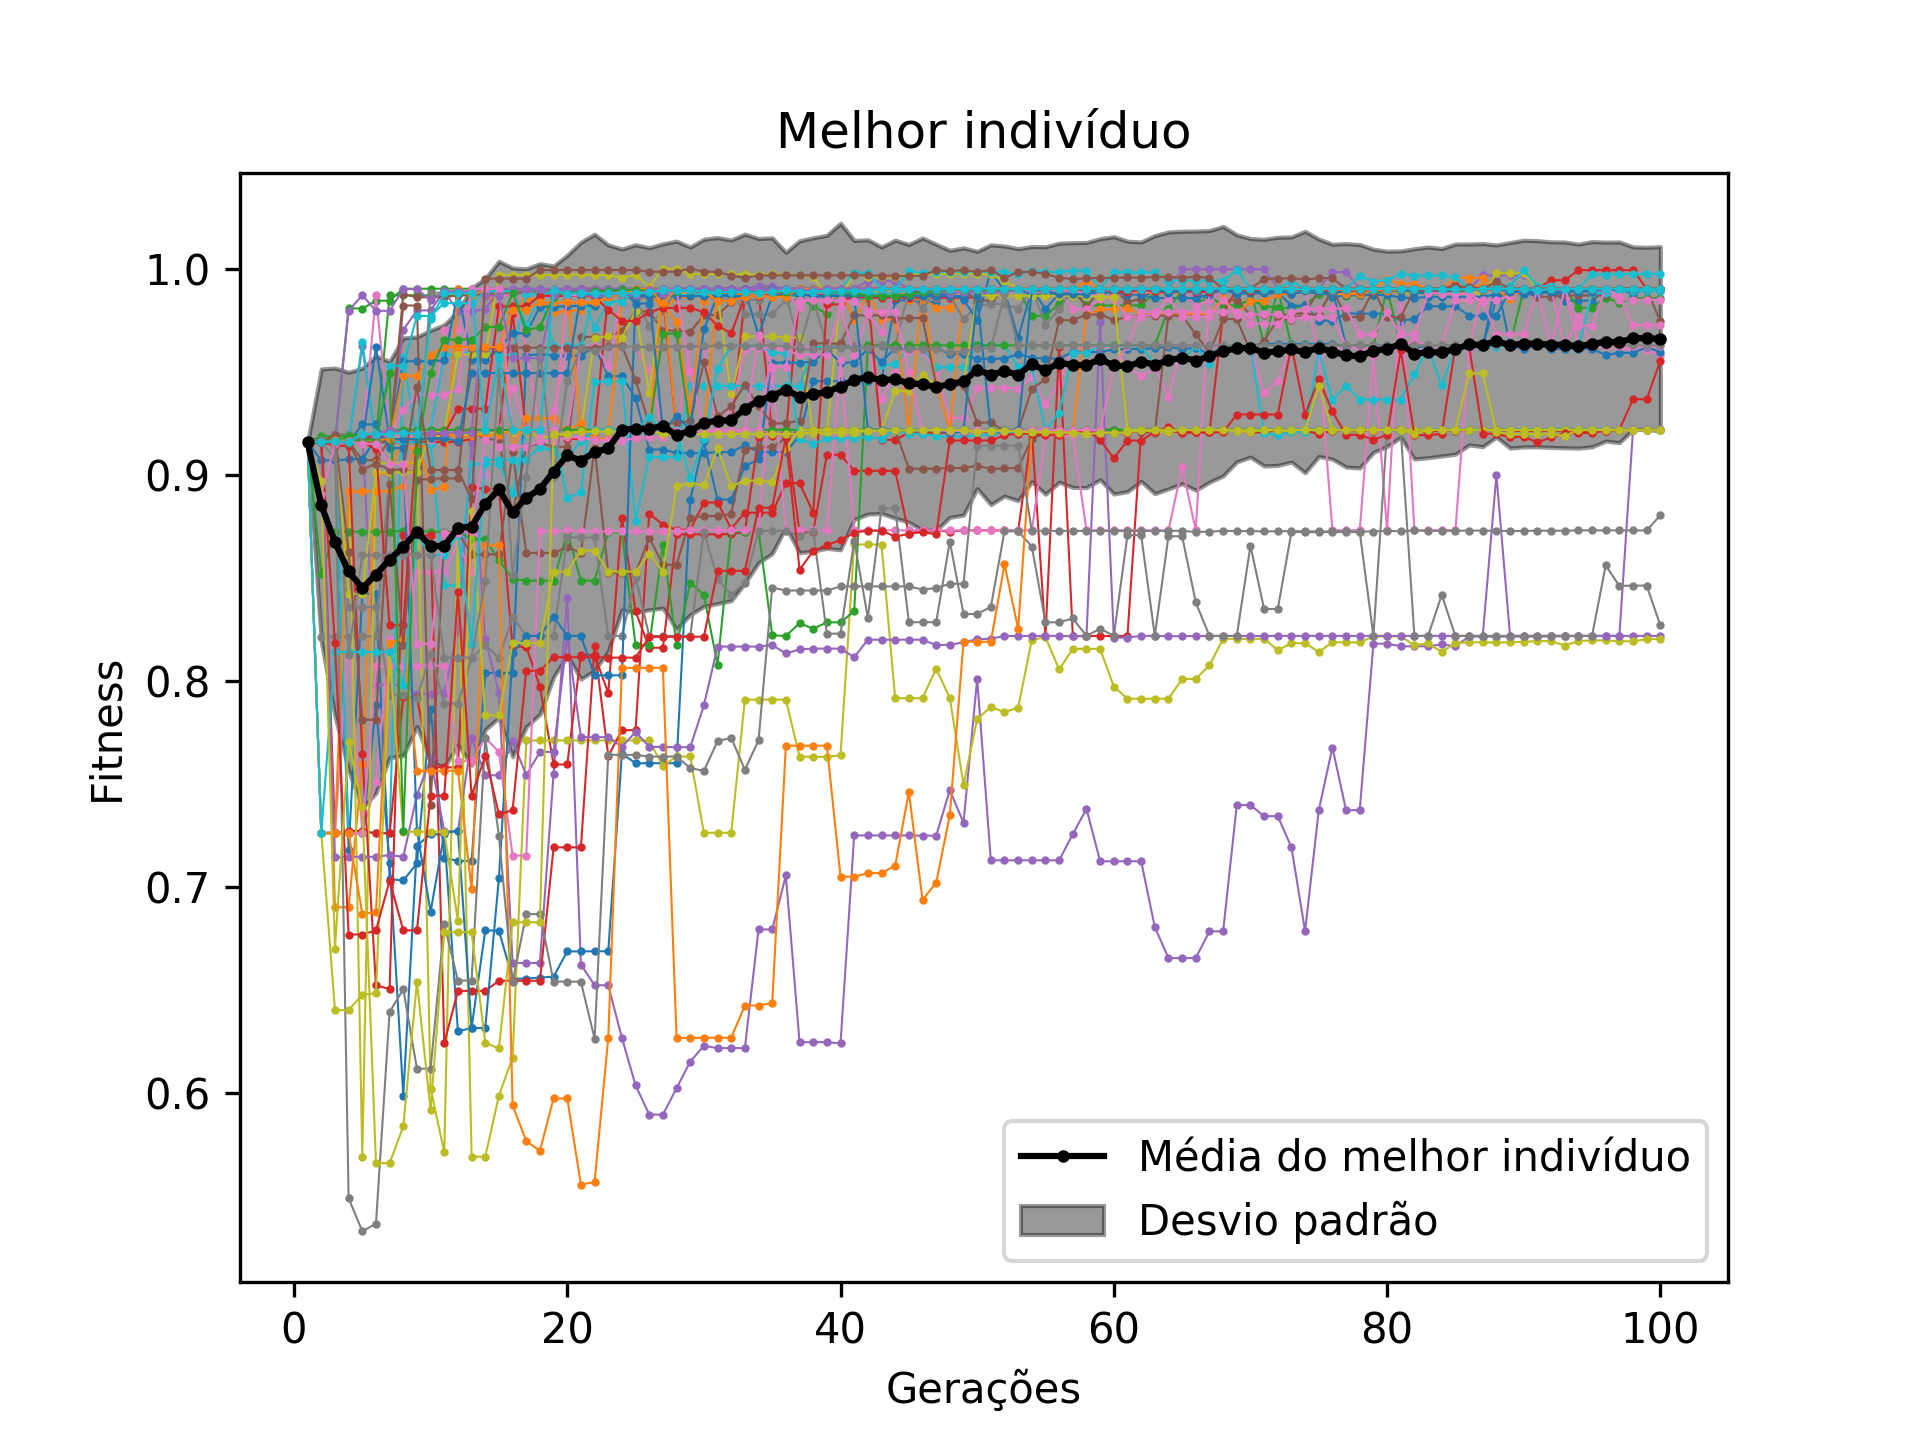
\includegraphics[width=1\textwidth]{sec-01/f6_none_fitness_vs_gen_best}
		\caption{Melhores indíviduos de todos os experimentos ao longo das gerações.
		Em preto é mostrado o comportamento médio dos 50 experimentos. }
	\end{subfigure}
	\hfill
	\begin{subfigure}{.45\textwidth}
		\centering
		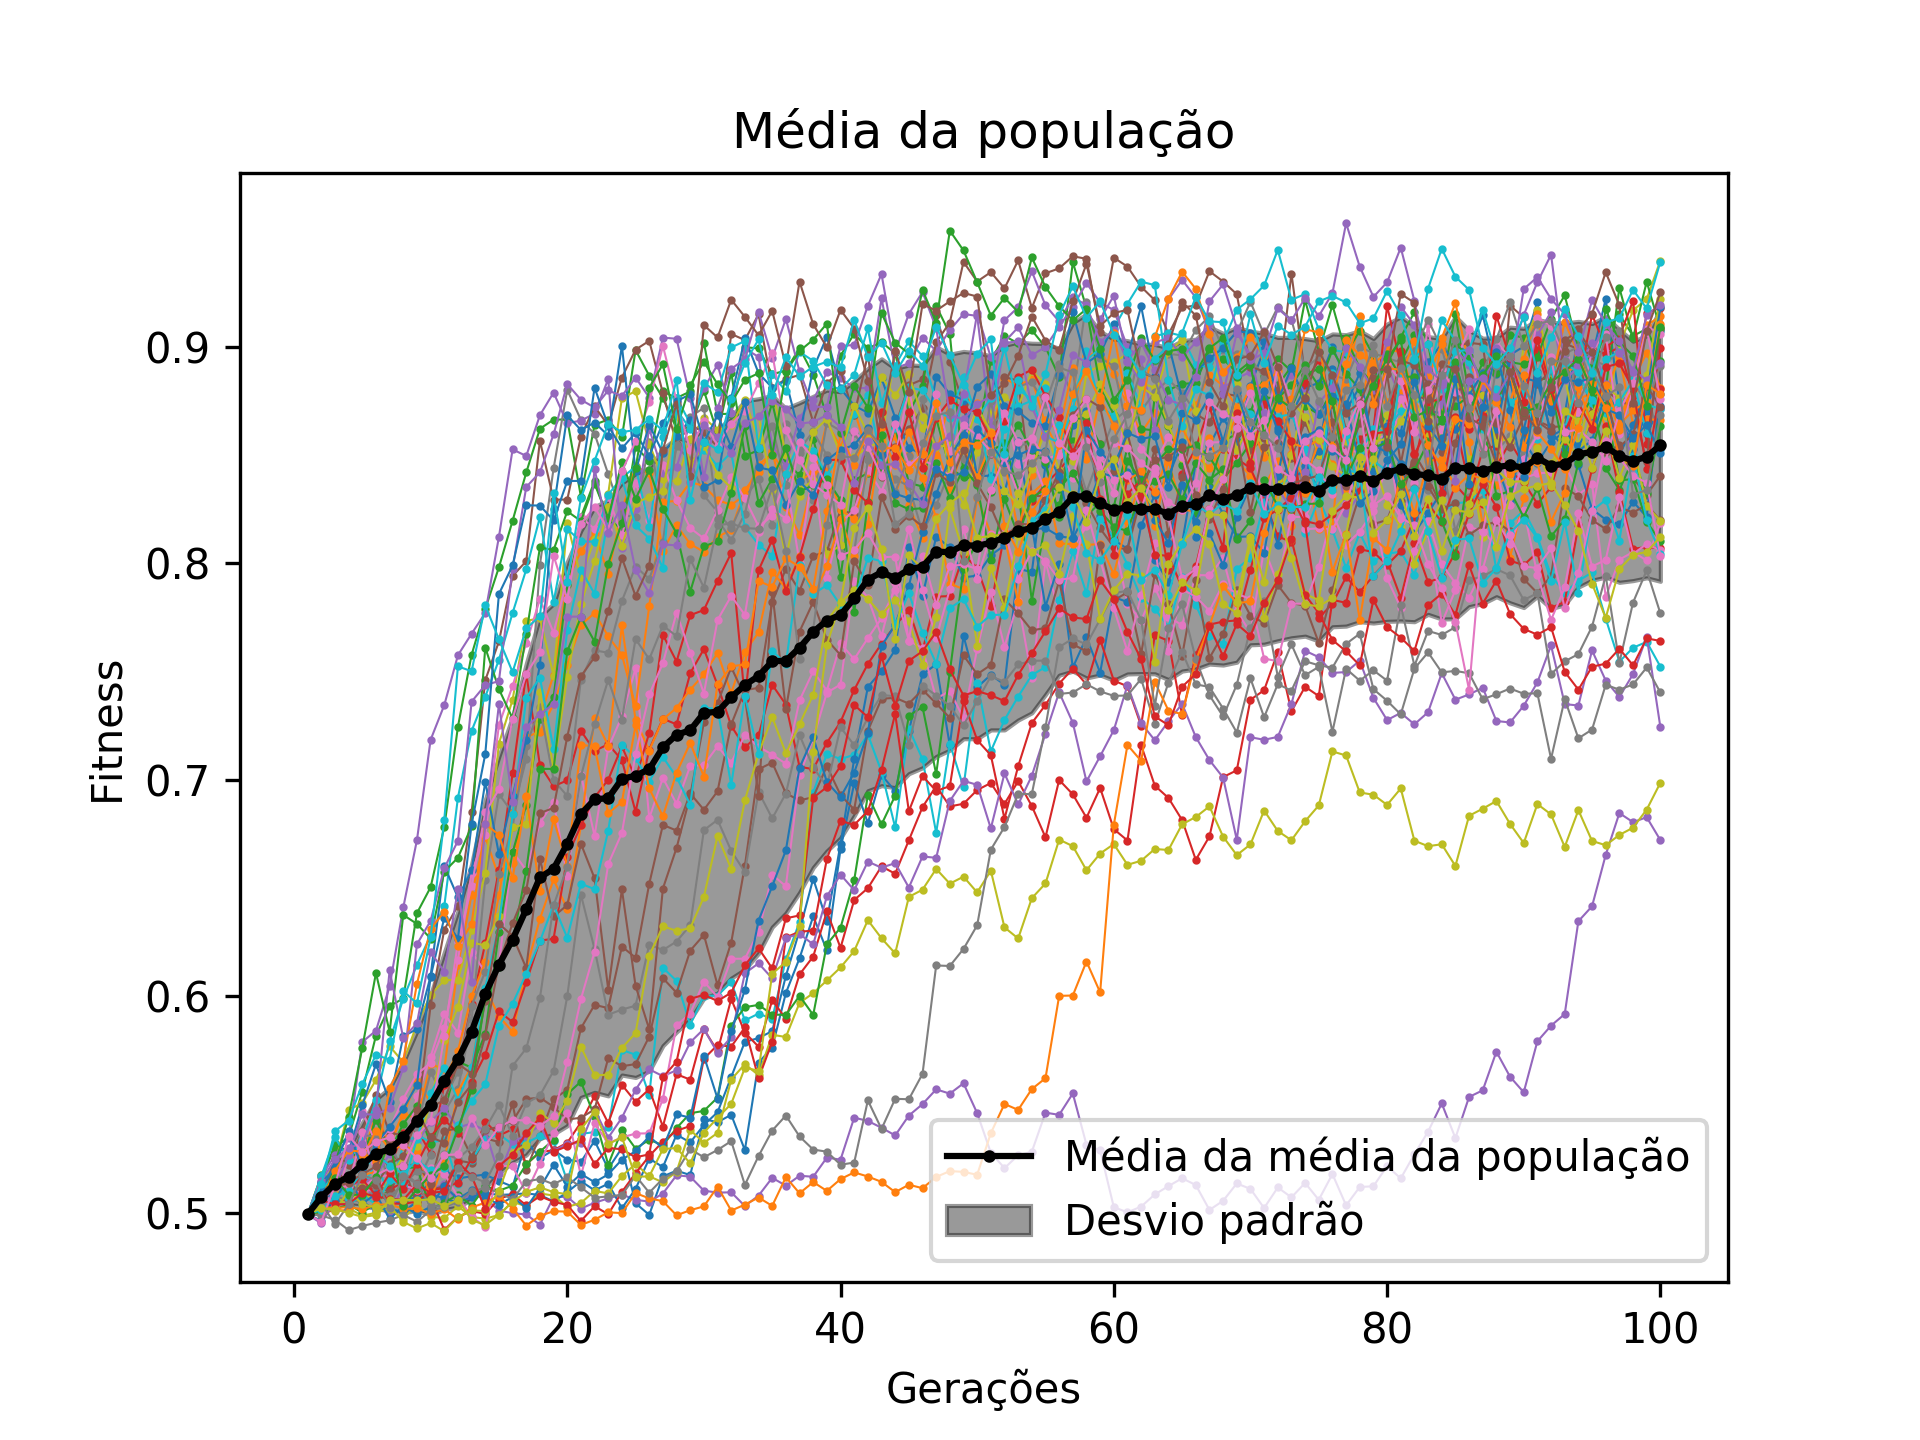
\includegraphics[width=1\textwidth]{sec-01/f6_none_fitness_vs_gen_pop}
		\caption{Média da população de todos os experimentos ao longo das gerações.
		Em preto é mostrado o comportamento médio dos 50 experimentos.}
	\end{subfigure}
	\caption{Resultados obtidos para a função $f6$ sem elitismo ou estado estacionário referentes ao teste 3 da tabela~\ref{tab:f6_none}}
\end{figure}

\begin{figure}[!htb]
	\begin{subfigure}{.45\textwidth}
		\centering
		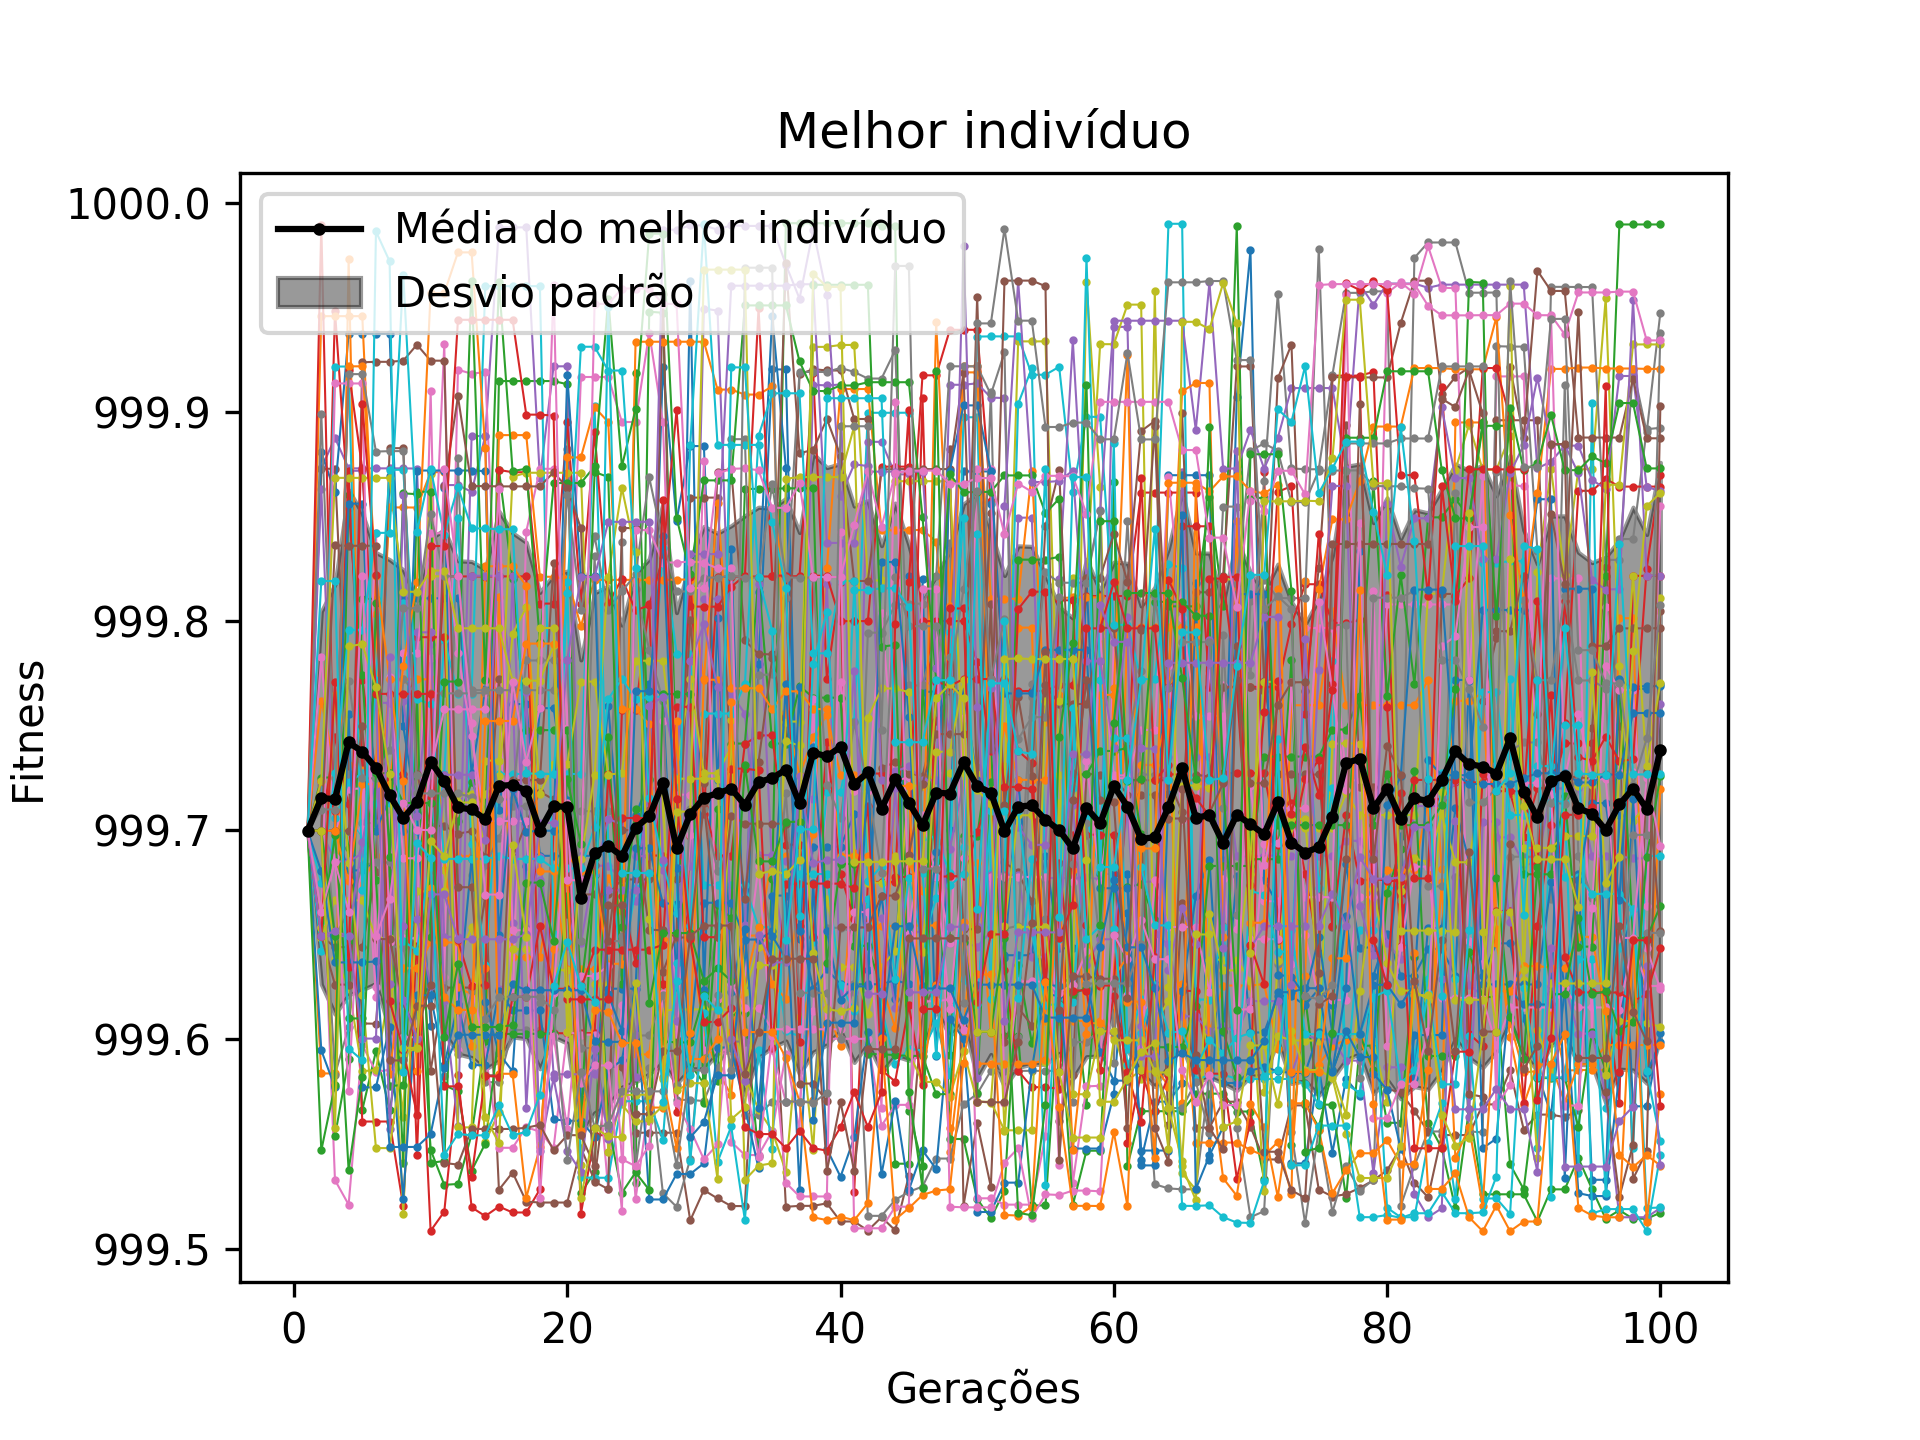
\includegraphics[width=1\textwidth]{sec-01/f6e_none_fitness_vs_gen_best}
		\caption{Melhores indíviduos de todos os experimentos ao longo das gerações.
		Em preto é mostrado o comportamento médio dos 50 experimentos. }
	\end{subfigure}
	\hfill
	\begin{subfigure}{.45\textwidth}
		\centering
		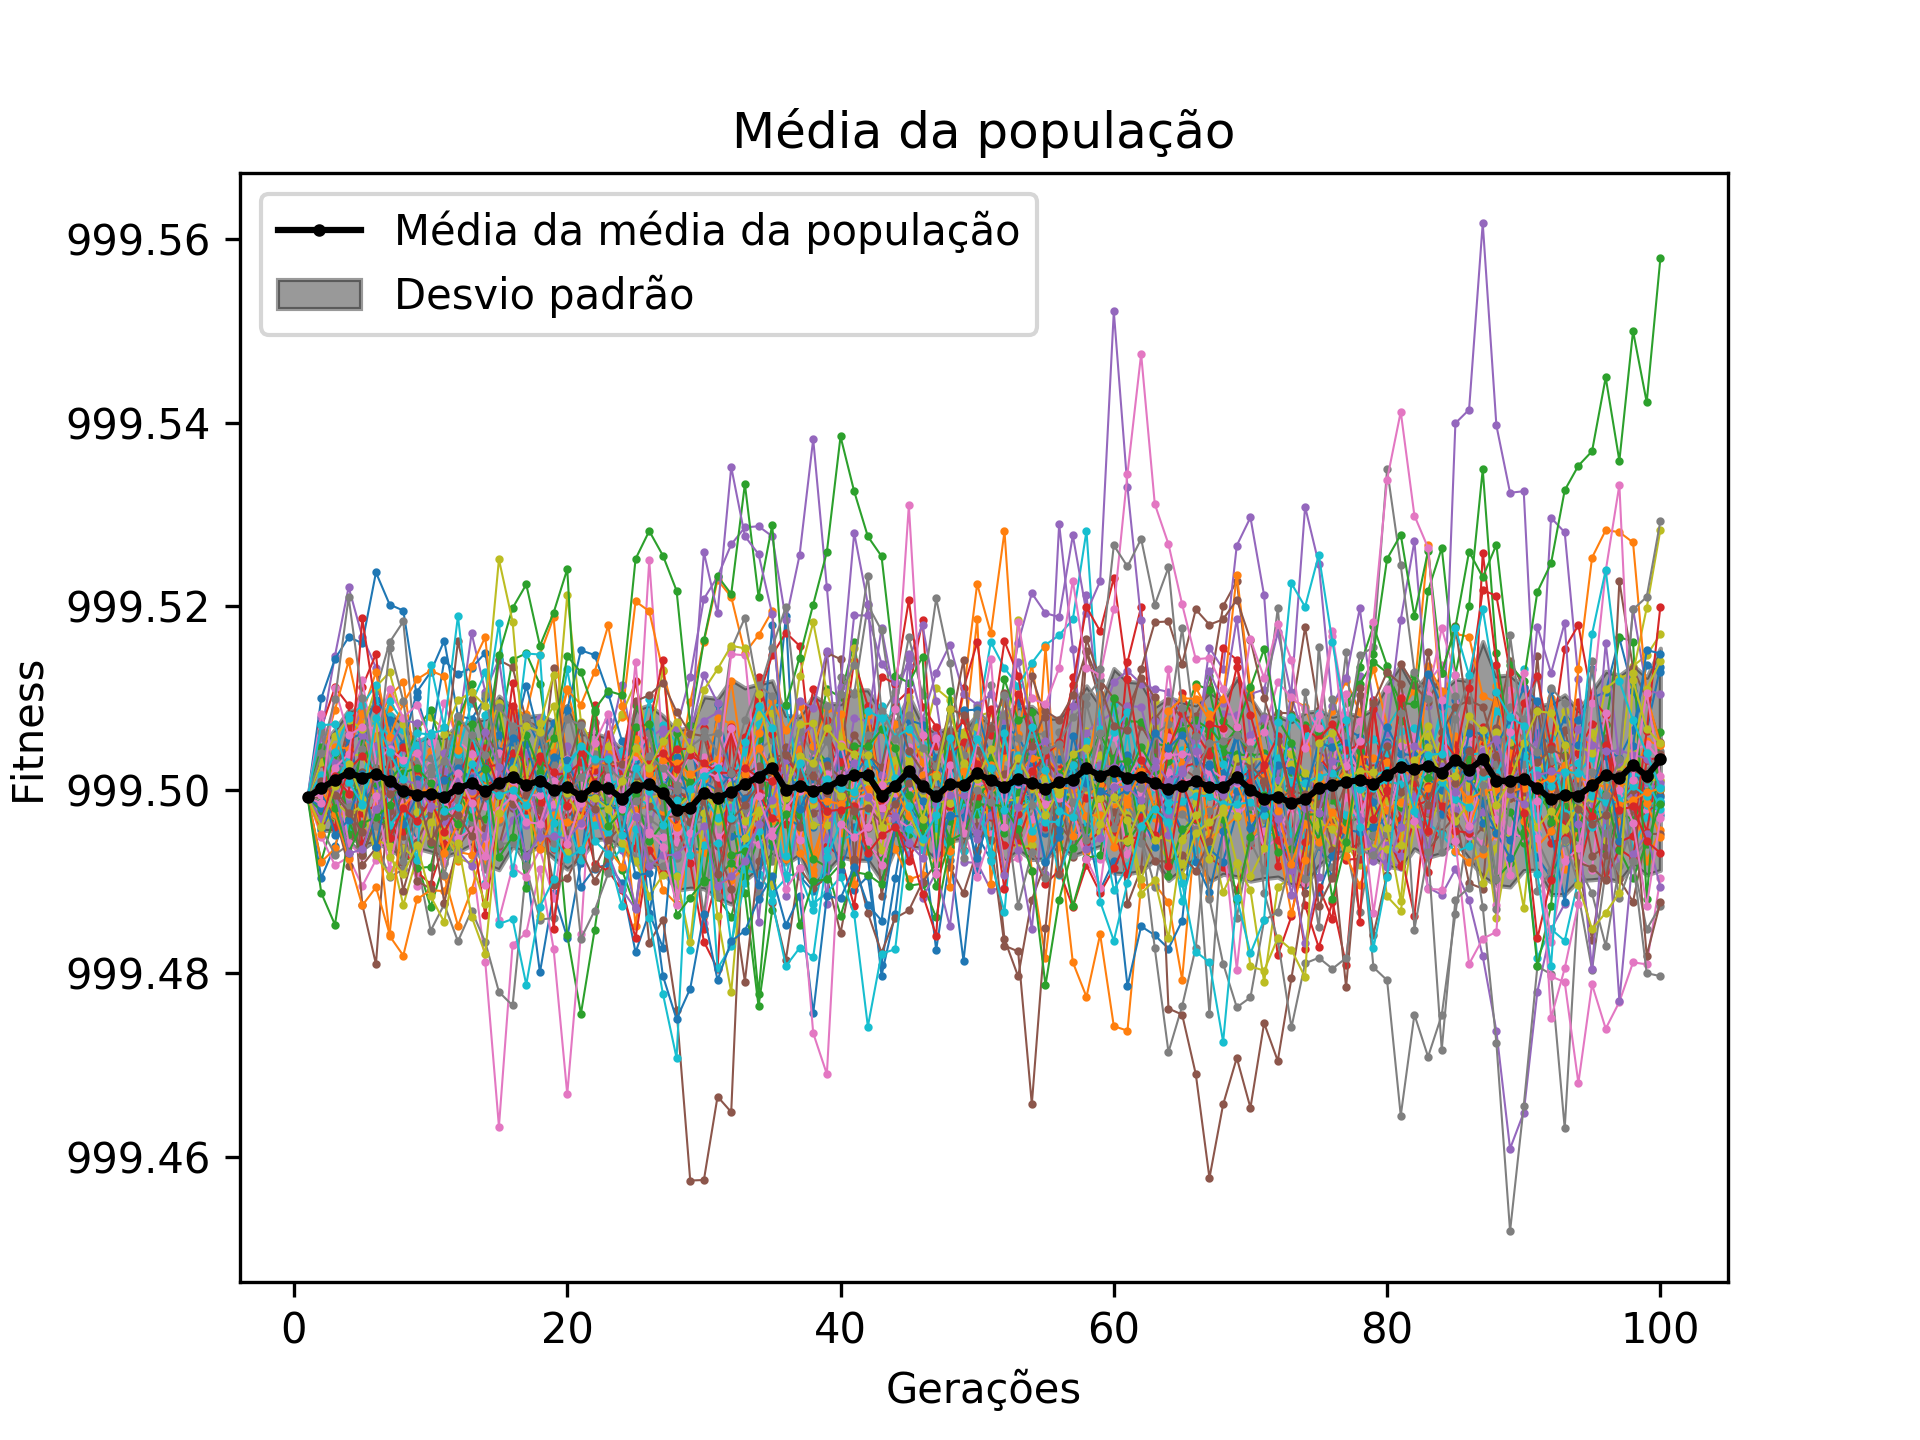
\includegraphics[width=1\textwidth]{sec-01/f6e_none_fitness_vs_gen_pop}
		\caption{Média da população de todos os experimentos ao longo das gerações.
		Em preto é mostrado o comportamento médio dos 50 experimentos.}
	\end{subfigure}
	\caption{Resultados obtidos para a função $f6_{elevada}$ sem elitismo ou estado estacionário referentes ao teste 1 da tabela~\ref{tab:f6_none}}
\end{figure}

\begin{figure}[!htb]
	\begin{subfigure}{.45\textwidth}
		\centering
		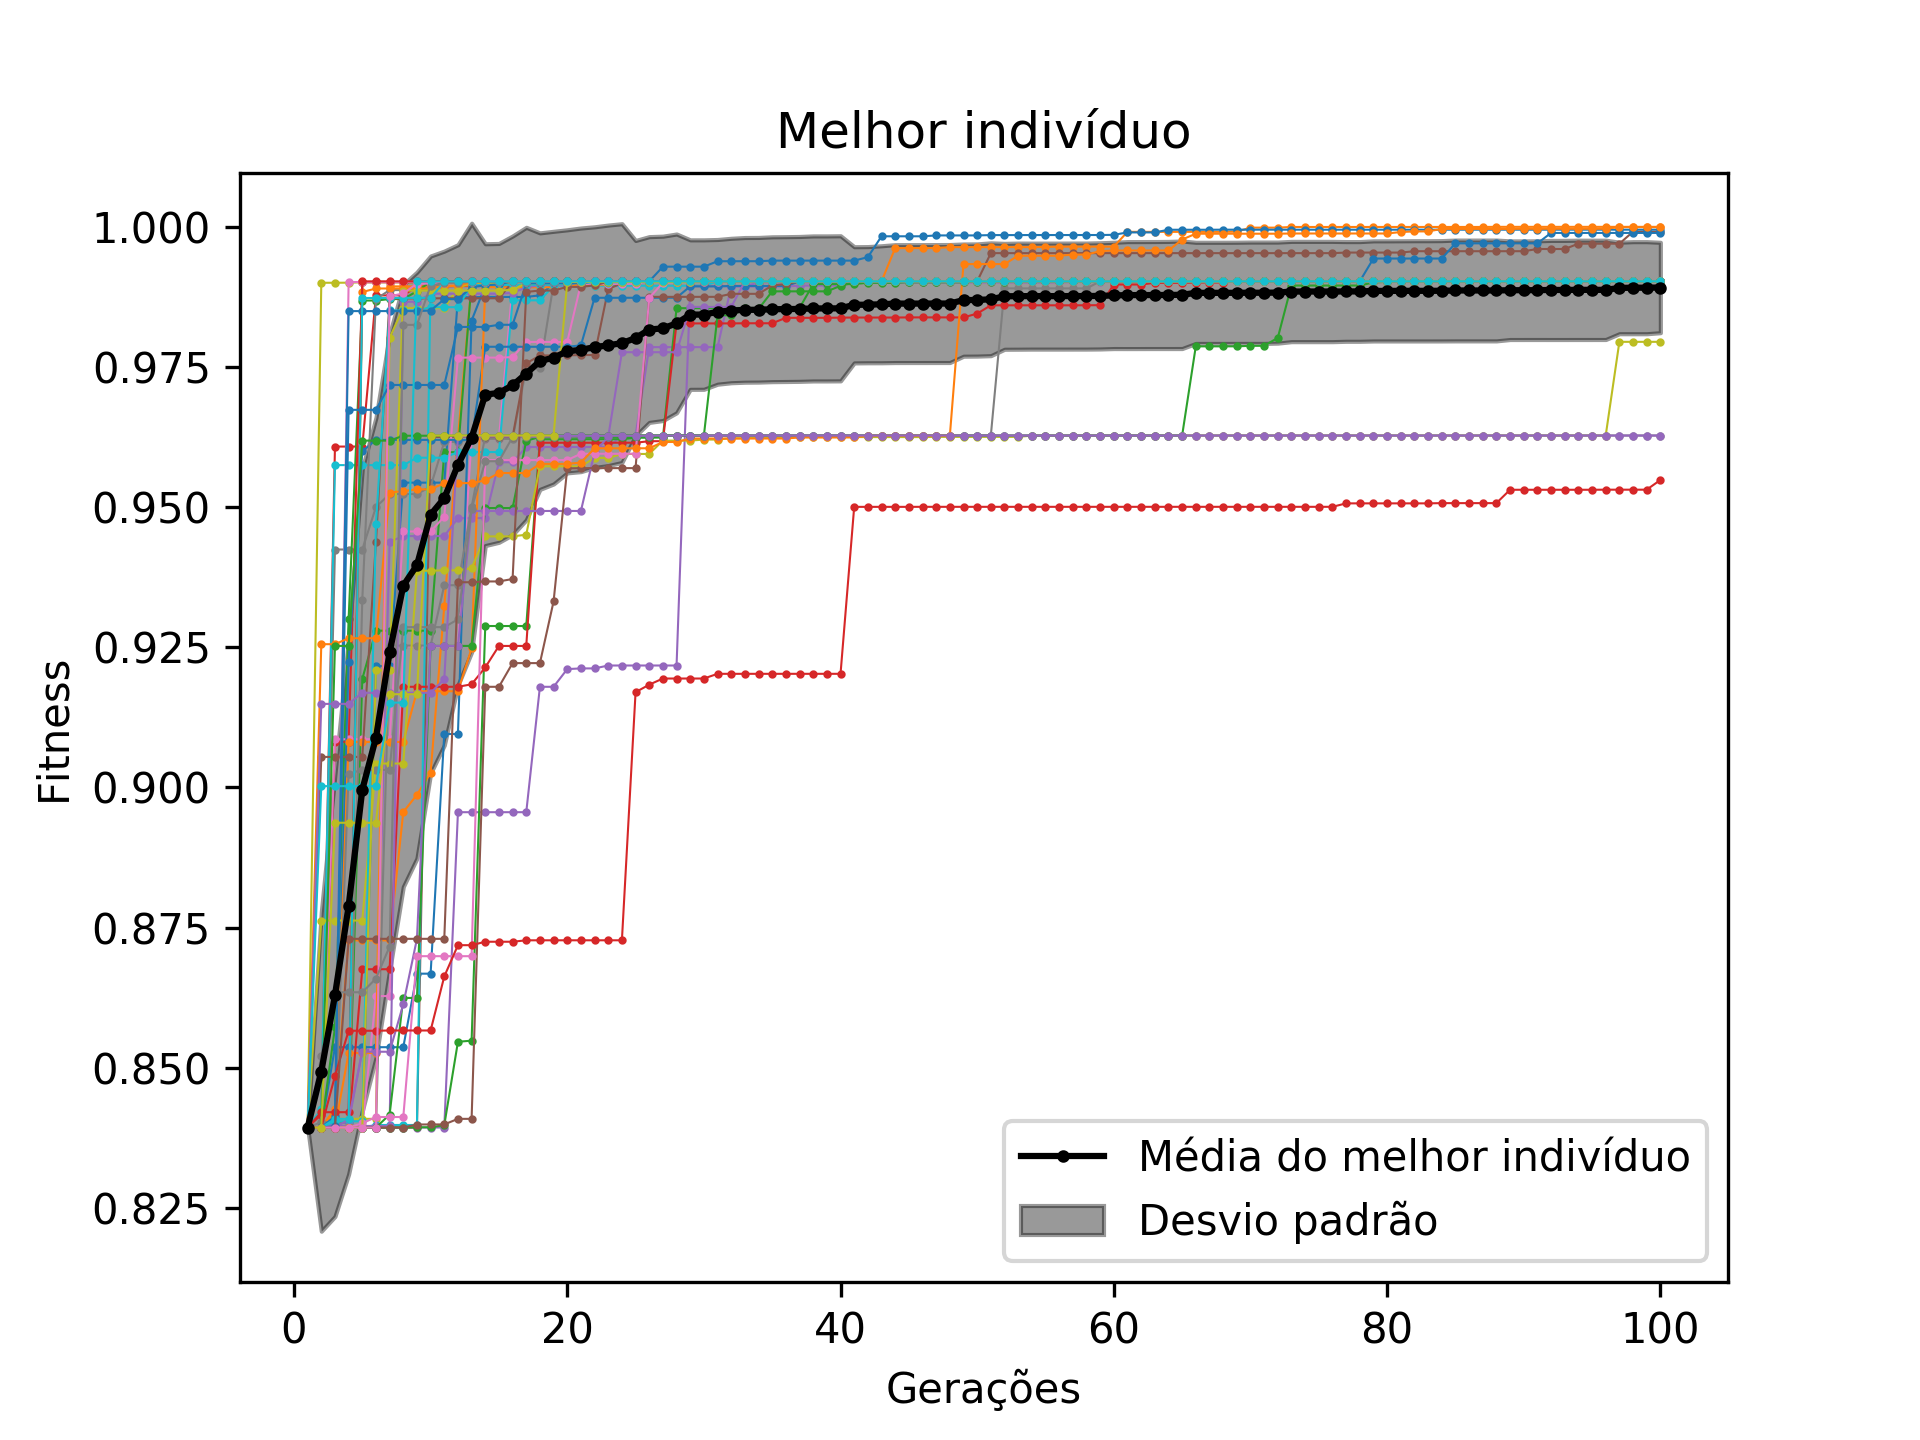
\includegraphics[width=1\textwidth]{sec-01/f6_elitist_fitness_vs_gen_best}
		\caption{Melhores indíviduos de todos os experimentos ao longo das gerações.
		Em preto é mostrado o comportamento médio dos 50 experimentos. }
	\end{subfigure}
	\hfill
	\begin{subfigure}{.45\textwidth}
		\centering
		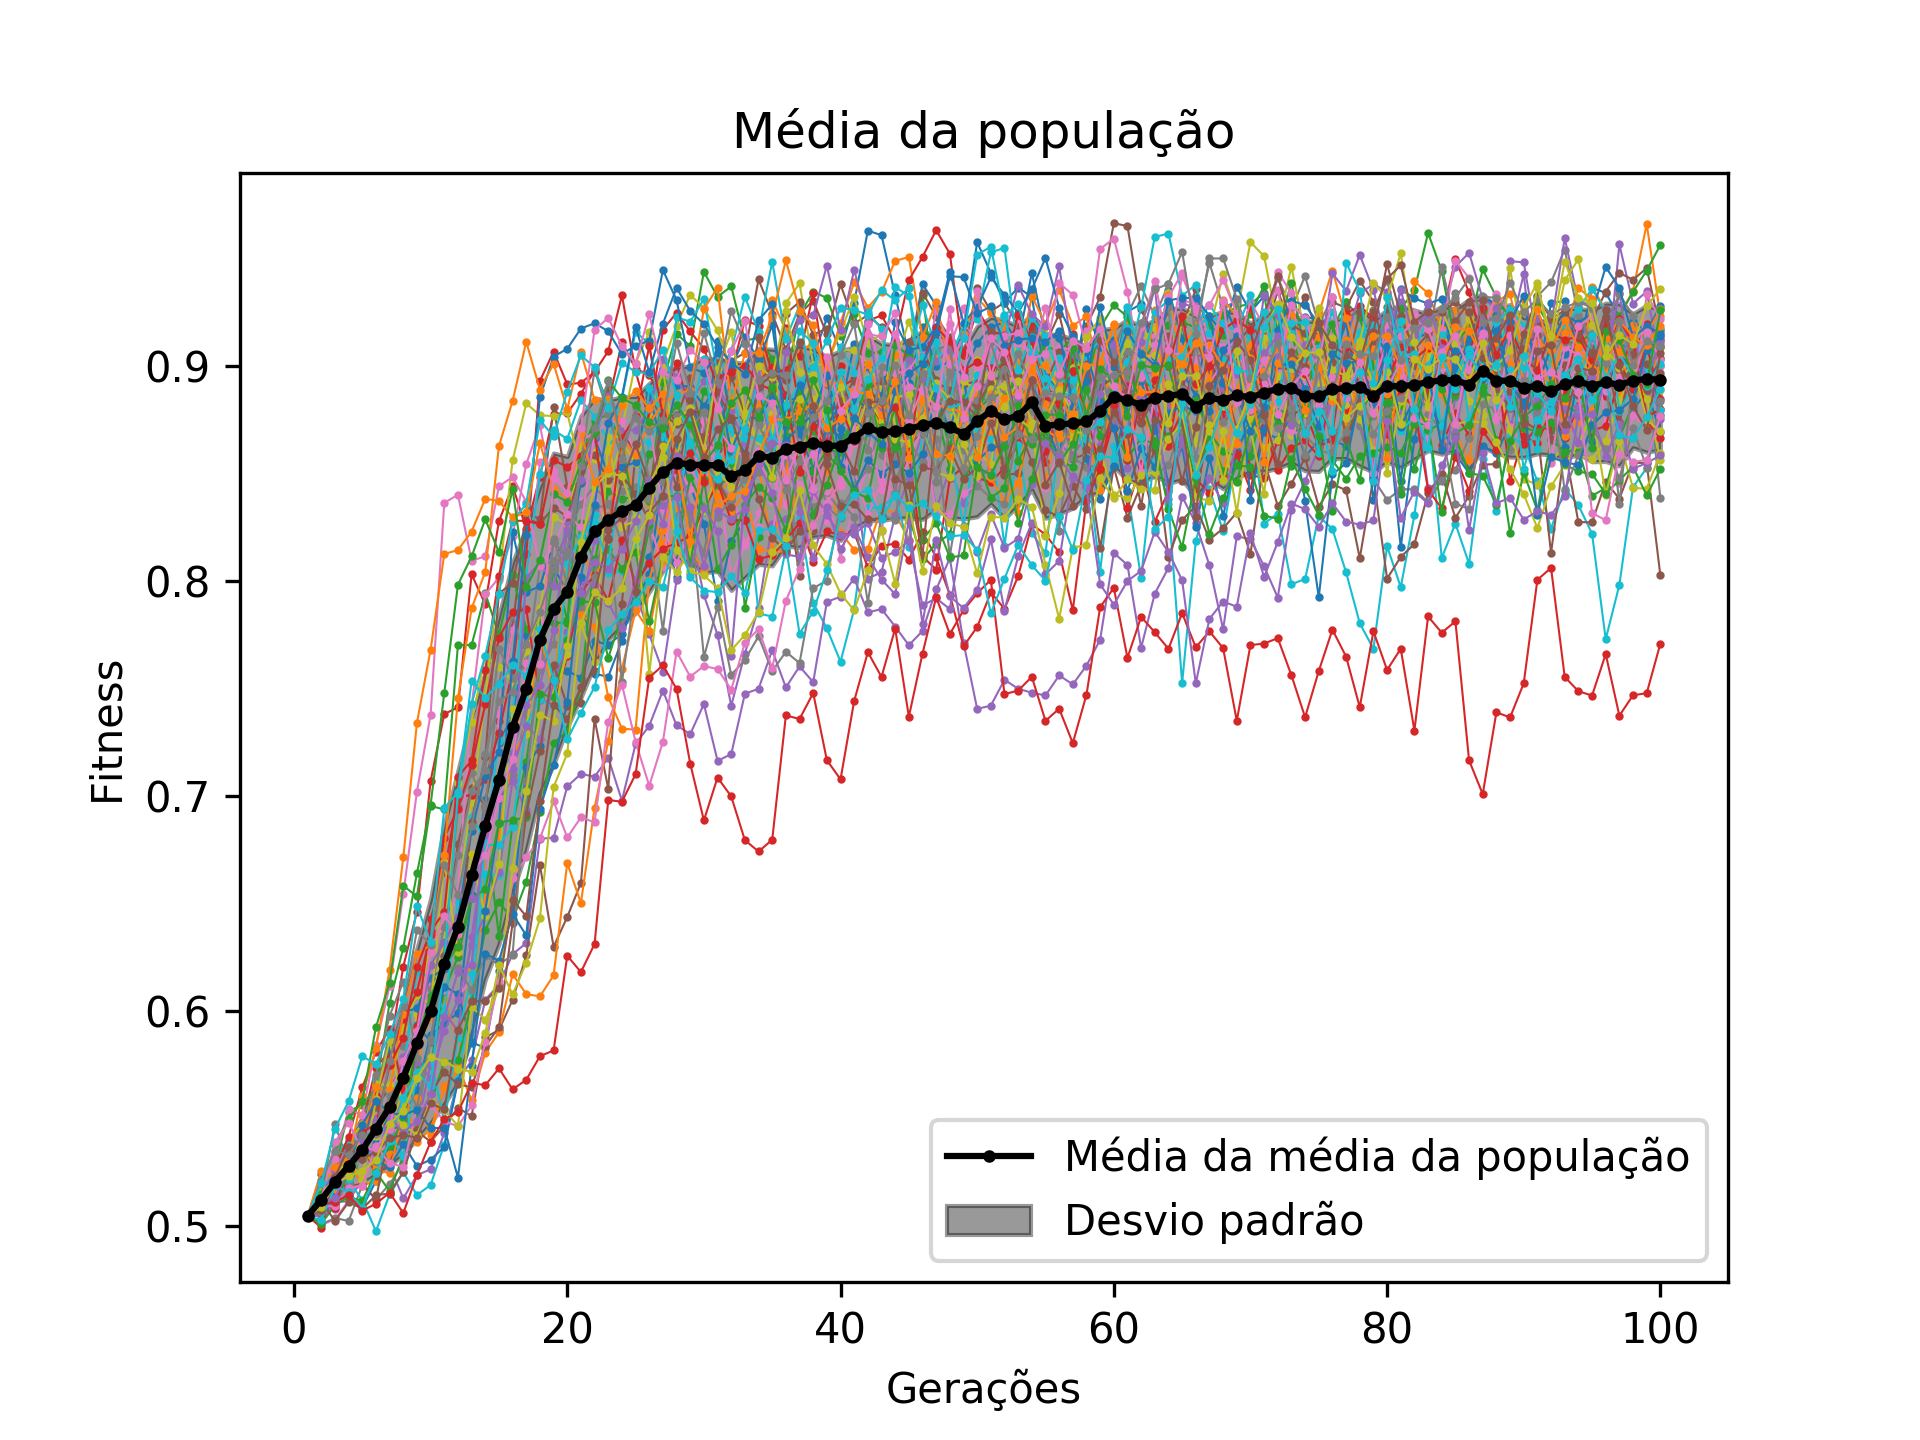
\includegraphics[width=1\textwidth]{sec-01/f6_elitist_fitness_vs_gen_pop}
		\caption{Média da população de todos os experimentos ao longo das gerações.
		Em preto é mostrado o comportamento médio dos 50 experimentos.}
	\end{subfigure}
	\caption{Resultados obtidos para a função $f6$ com elitismo referentes ao teste 5 da tabela~\ref{tab:f6_elitist}}
\end{figure}

\begin{figure}[!htb]
	\begin{subfigure}{.45\textwidth}
		\centering
		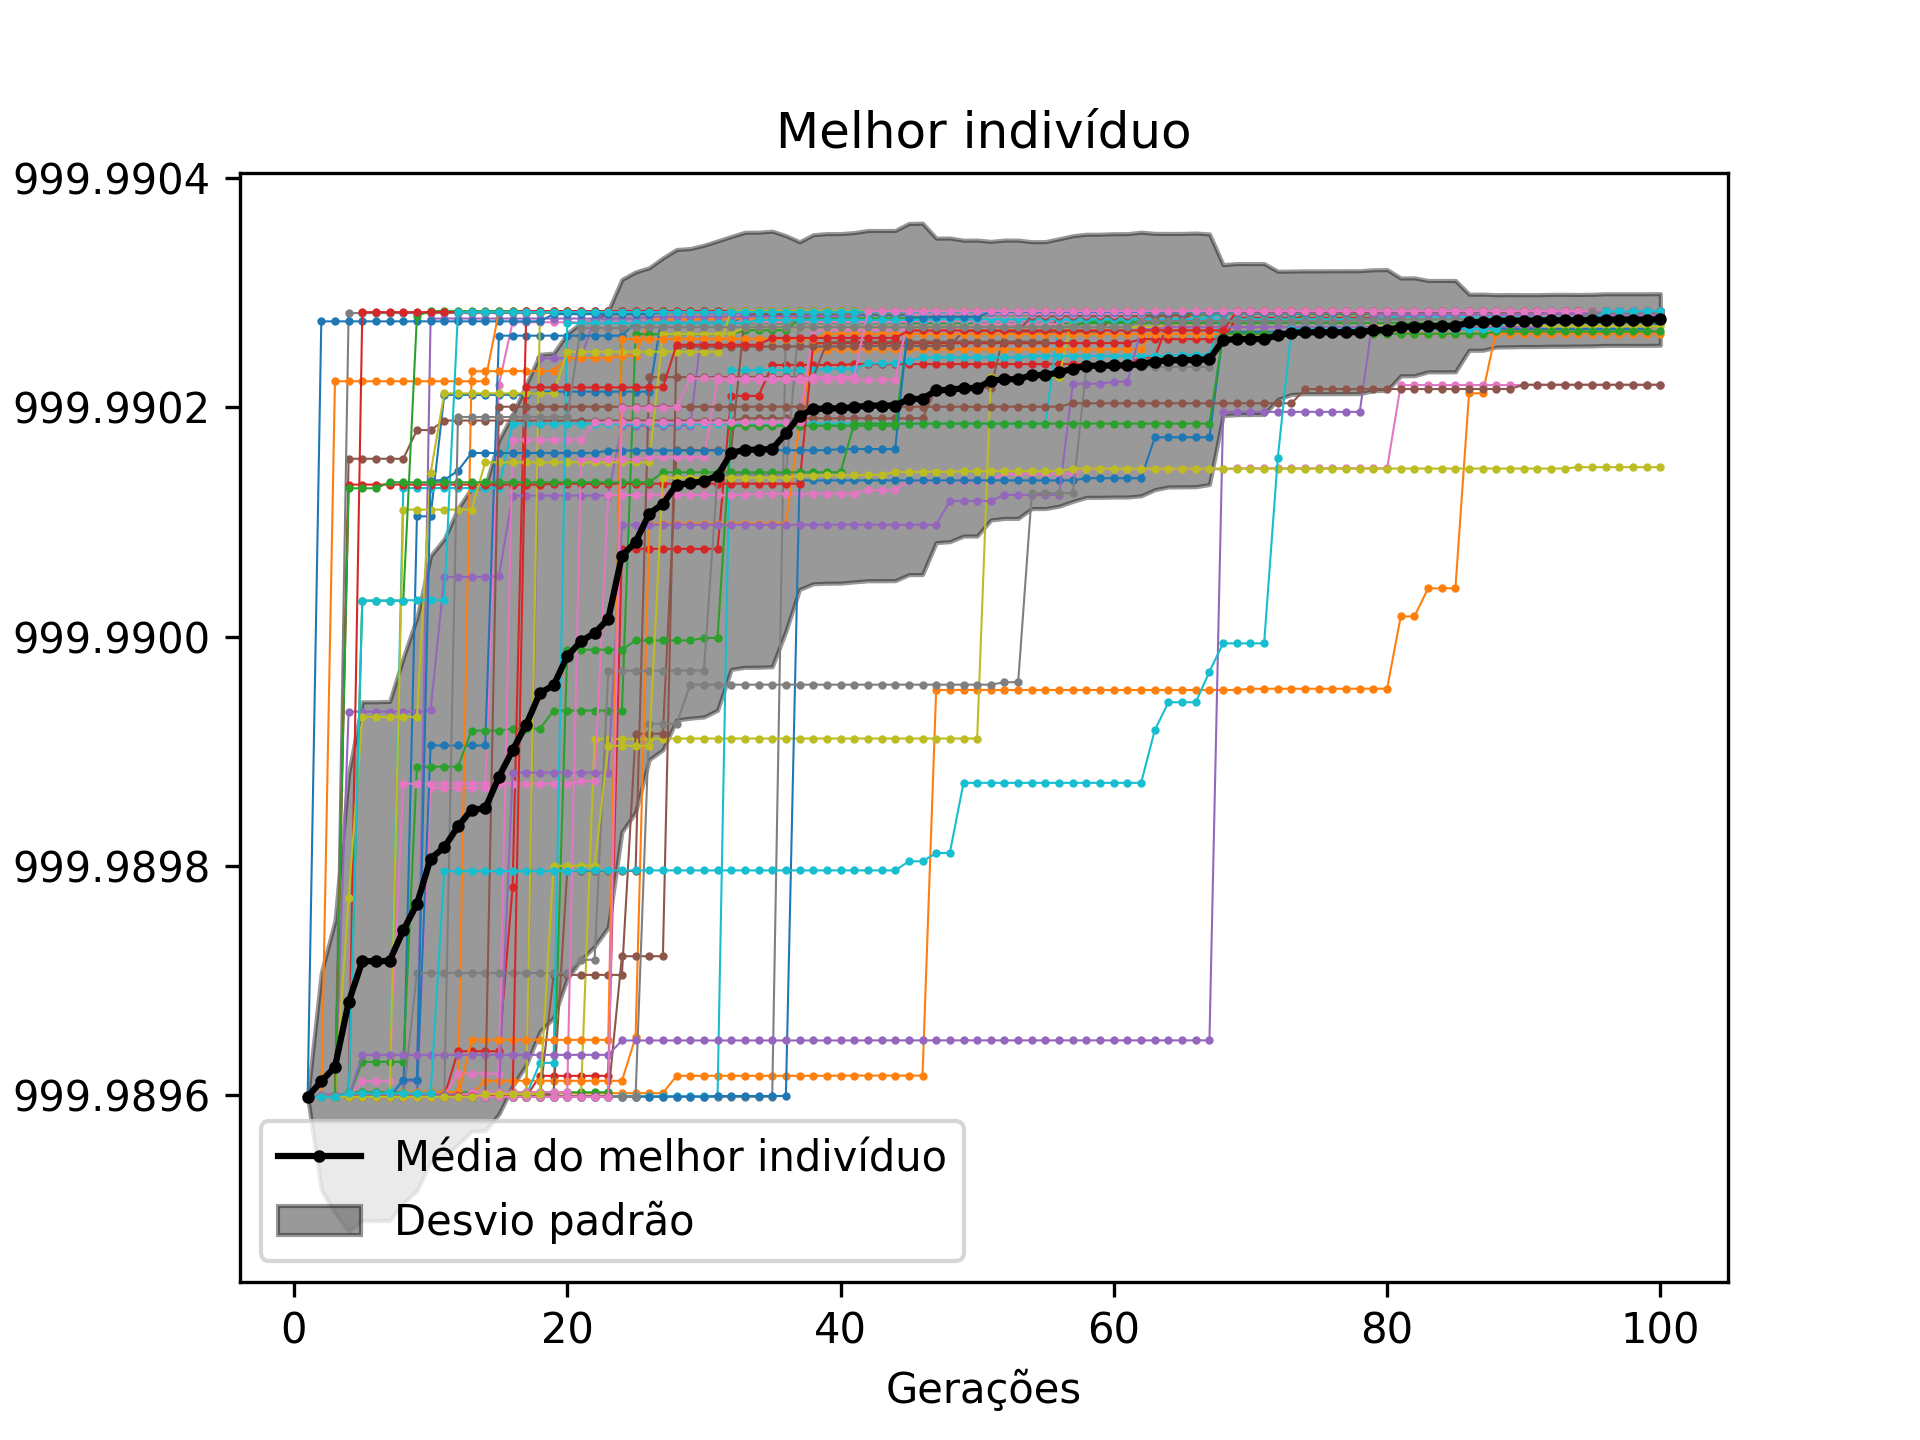
\includegraphics[width=1\textwidth]{sec-01/f6e_elitist_fitness_vs_gen_best}
		\caption{Melhores indíviduos de todos os experimentos ao longo das gerações.
		Em preto é mostrado o comportamento médio dos 50 experimentos. }
	\end{subfigure}
	\hfill
	\begin{subfigure}{.45\textwidth}
		\centering
		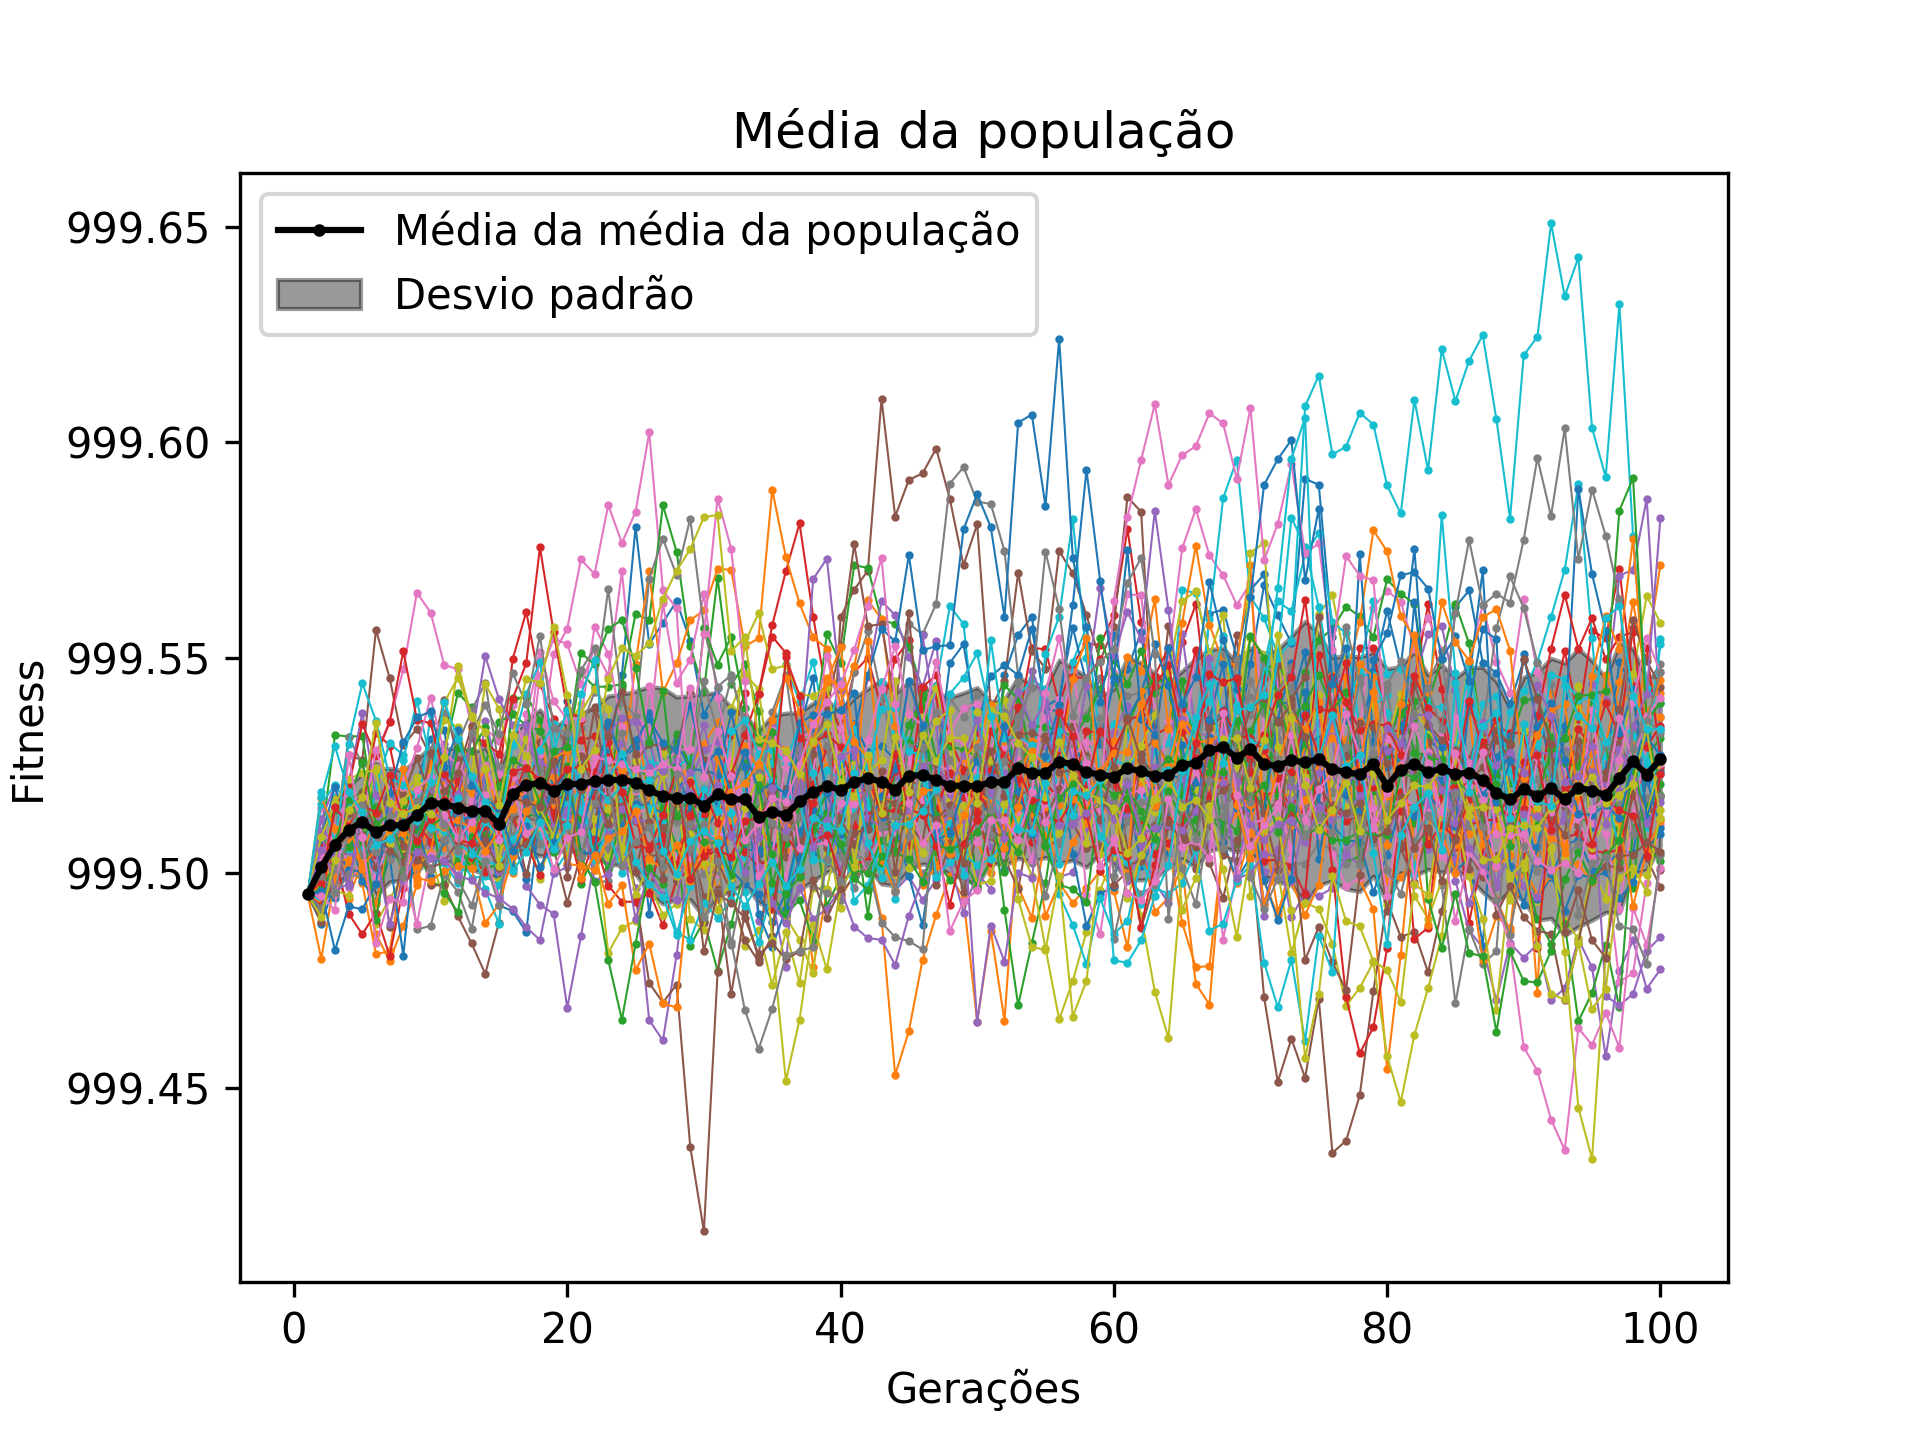
\includegraphics[width=1\textwidth]{sec-01/f6e_elitist_fitness_vs_gen_pop}
		\caption{Média da população de todos os experimentos ao longo das gerações.
		Em preto é mostrado o comportamento médio dos 50 experimentos.}
	\end{subfigure}
	\caption{Resultados obtidos para a função $f6_{elevada}$ com elitismo referentes ao teste 3 da tabela~\ref{tab:f6_elitist}}
\end{figure}

	Posteriormente, utilizando a elitismo e estado estacionário obtiveram-se um aumento de performance tanto para a função
	$f6$ quanto para a função $f6_{elevada}$. Os resultados obtidos são apresentados nas tabelas~\ref{tab:f6_elitist}
	e \ref{tab:f6_stationary}.

	\begin{table}[!htb]
		\centering
		\begin{tabular}{|c|c|c|c|c|}
			\hline
			\rowcolor[HTML]{9B9B9B}
			& \multicolumn{2}{c}{Função F6} & \multicolumn{2}{c}{Função F6 elevada} \\
			\rowcolor[HTML]{9B9B9B}
			Teste & Média melhor indíviduo & Média população & Média melhor indíviduo & Média população \\\hline
			1 & 0.98518 & 0.88408 & 999.99028 & 999.52910 \\\hline
			2 & 0.97977 & 0.87092 & 999.98128 & 999.52672 \\\hline
			3 & 0.97706 & 0.86914 & 999.98433 & 999.53551 \\\hline
			4 & 0.97921 & 0.87249 & 999.98058 & 999.52753 \\\hline
			5 & 0.98918 & 0.89792 & 999.98472 & 999.52755 \\\hline
			\textbf{Média Final} & \textbf{0.98208} & \textbf{0.87891} & \textbf{999.98424} & \textbf{999.5293} \\\hline
		\end{tabular}
		\caption{Resultados da função $f6$ e $f6_{elevada}$ com elitismo. \label{tab:f6_elitist}}
	\end{table}

	\begin{table}[!htb]
		\centering
		\begin{tabular}{|c|c|c|c|c|}
			\hline
			\rowcolor[HTML]{9B9B9B}
			& \multicolumn{2}{c}{Função F6} & \multicolumn{2}{c}{Função F6 elevada} \\
			\rowcolor[HTML]{9B9B9B}
			Teste & Média melhor indíviduo & Média população & Média melhor indíviduo & Média população \\\hline
			1 & 0.96897 & 0.95154 & 999.98164 & 999.96859 \\\hline
			2 & 0.96789 & 0.95841 & 999.95580 & 999.93493 \\\hline
			3 & 0.97028 & 0.95798 & 999.96191 & 999.94779 \\\hline
			4 & 0.98858 & 0.98103 & 999.98187 & 999.96661 \\\hline
			5 & 0.96920 & 0.95792 & 999.97647 & 999.95859 \\\hline
			\textbf{Média Final} & \textbf{0.97298} & \textbf{0.96138} & \textbf{999.97154} & \textbf{999.95530} \\\hline
		\end{tabular}
		\caption{Resultados da função $f6$ e $f6_{elevada}$ com estado estacionário de 20\% \label{tab:f6_stationary}}
	\end{table}

	\begin{figure}[!htb]
		\begin{subfigure}{.45\textwidth}
			\centering
			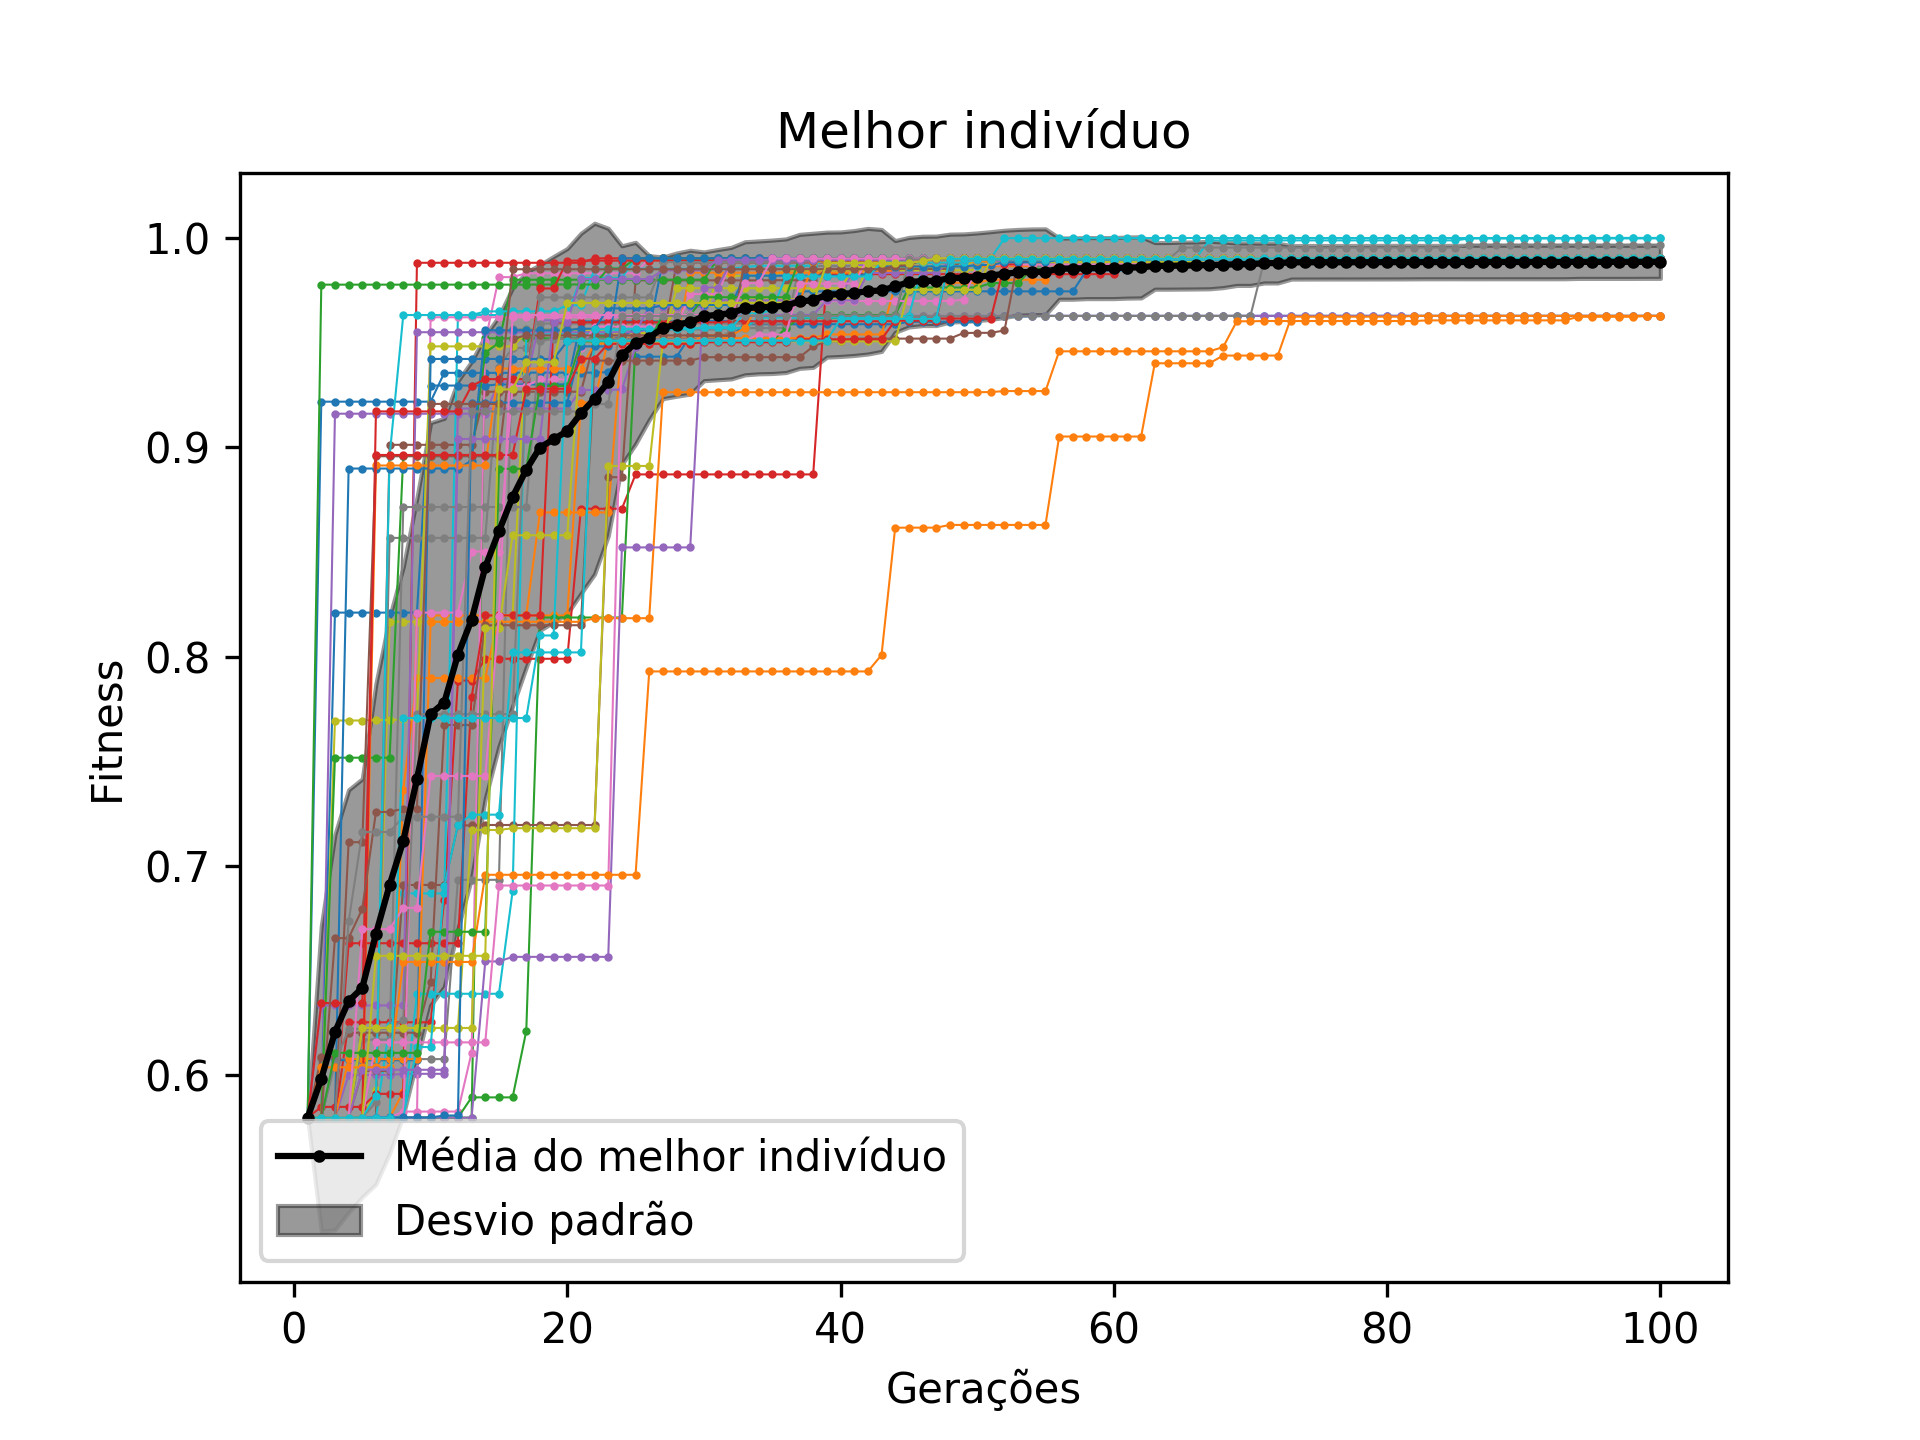
\includegraphics[width=1\textwidth]{sec-01/f6_ss_fitness_vs_gen_best}
			\caption{Melhores indíviduos de todos os experimentos ao longo das gerações.
			Em preto é mostrado o comportamento médio dos 50 experimentos. }
		\end{subfigure}
		\hfill
		\begin{subfigure}{.45\textwidth}
			\centering
			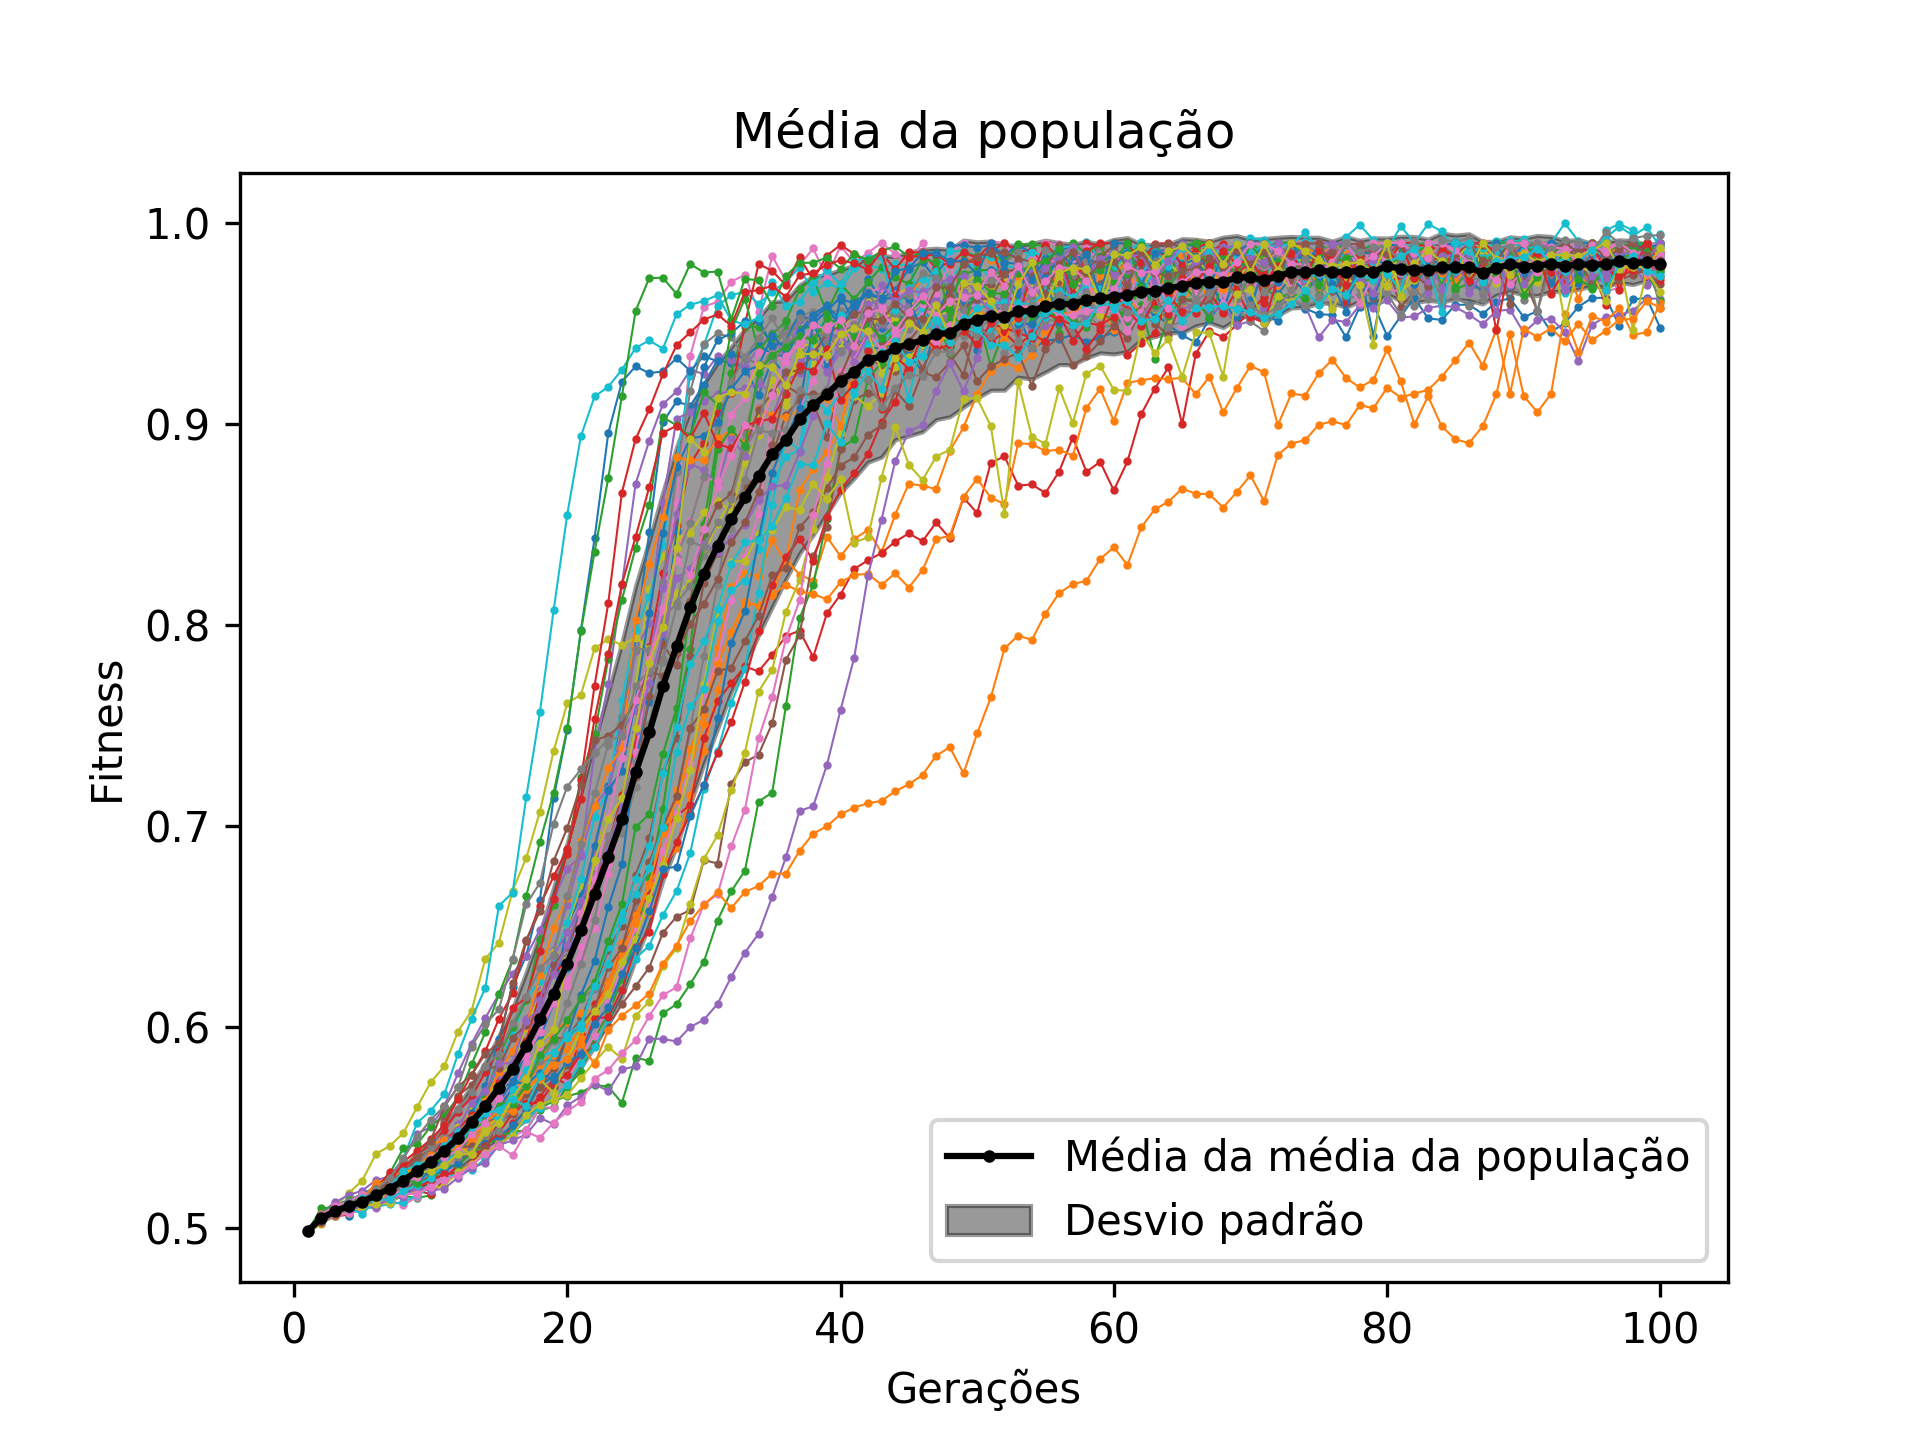
\includegraphics[width=1\textwidth]{sec-01/f6_ss_fitness_vs_gen_pop}
			\caption{Média da população de todos os experimentos ao longo das gerações.
			Em preto é mostrado o comportamento médio dos 50 experimentos.}
		\end{subfigure}
		\caption{Resultados obtidos para a função $f6$ com estado estacionário de 20\% referentes ao teste 4 da tabela~\ref{tab:f6_stationary}}
	\end{figure}

	\begin{figure}[!htb]
		\begin{subfigure}{.45\textwidth}
			\centering
			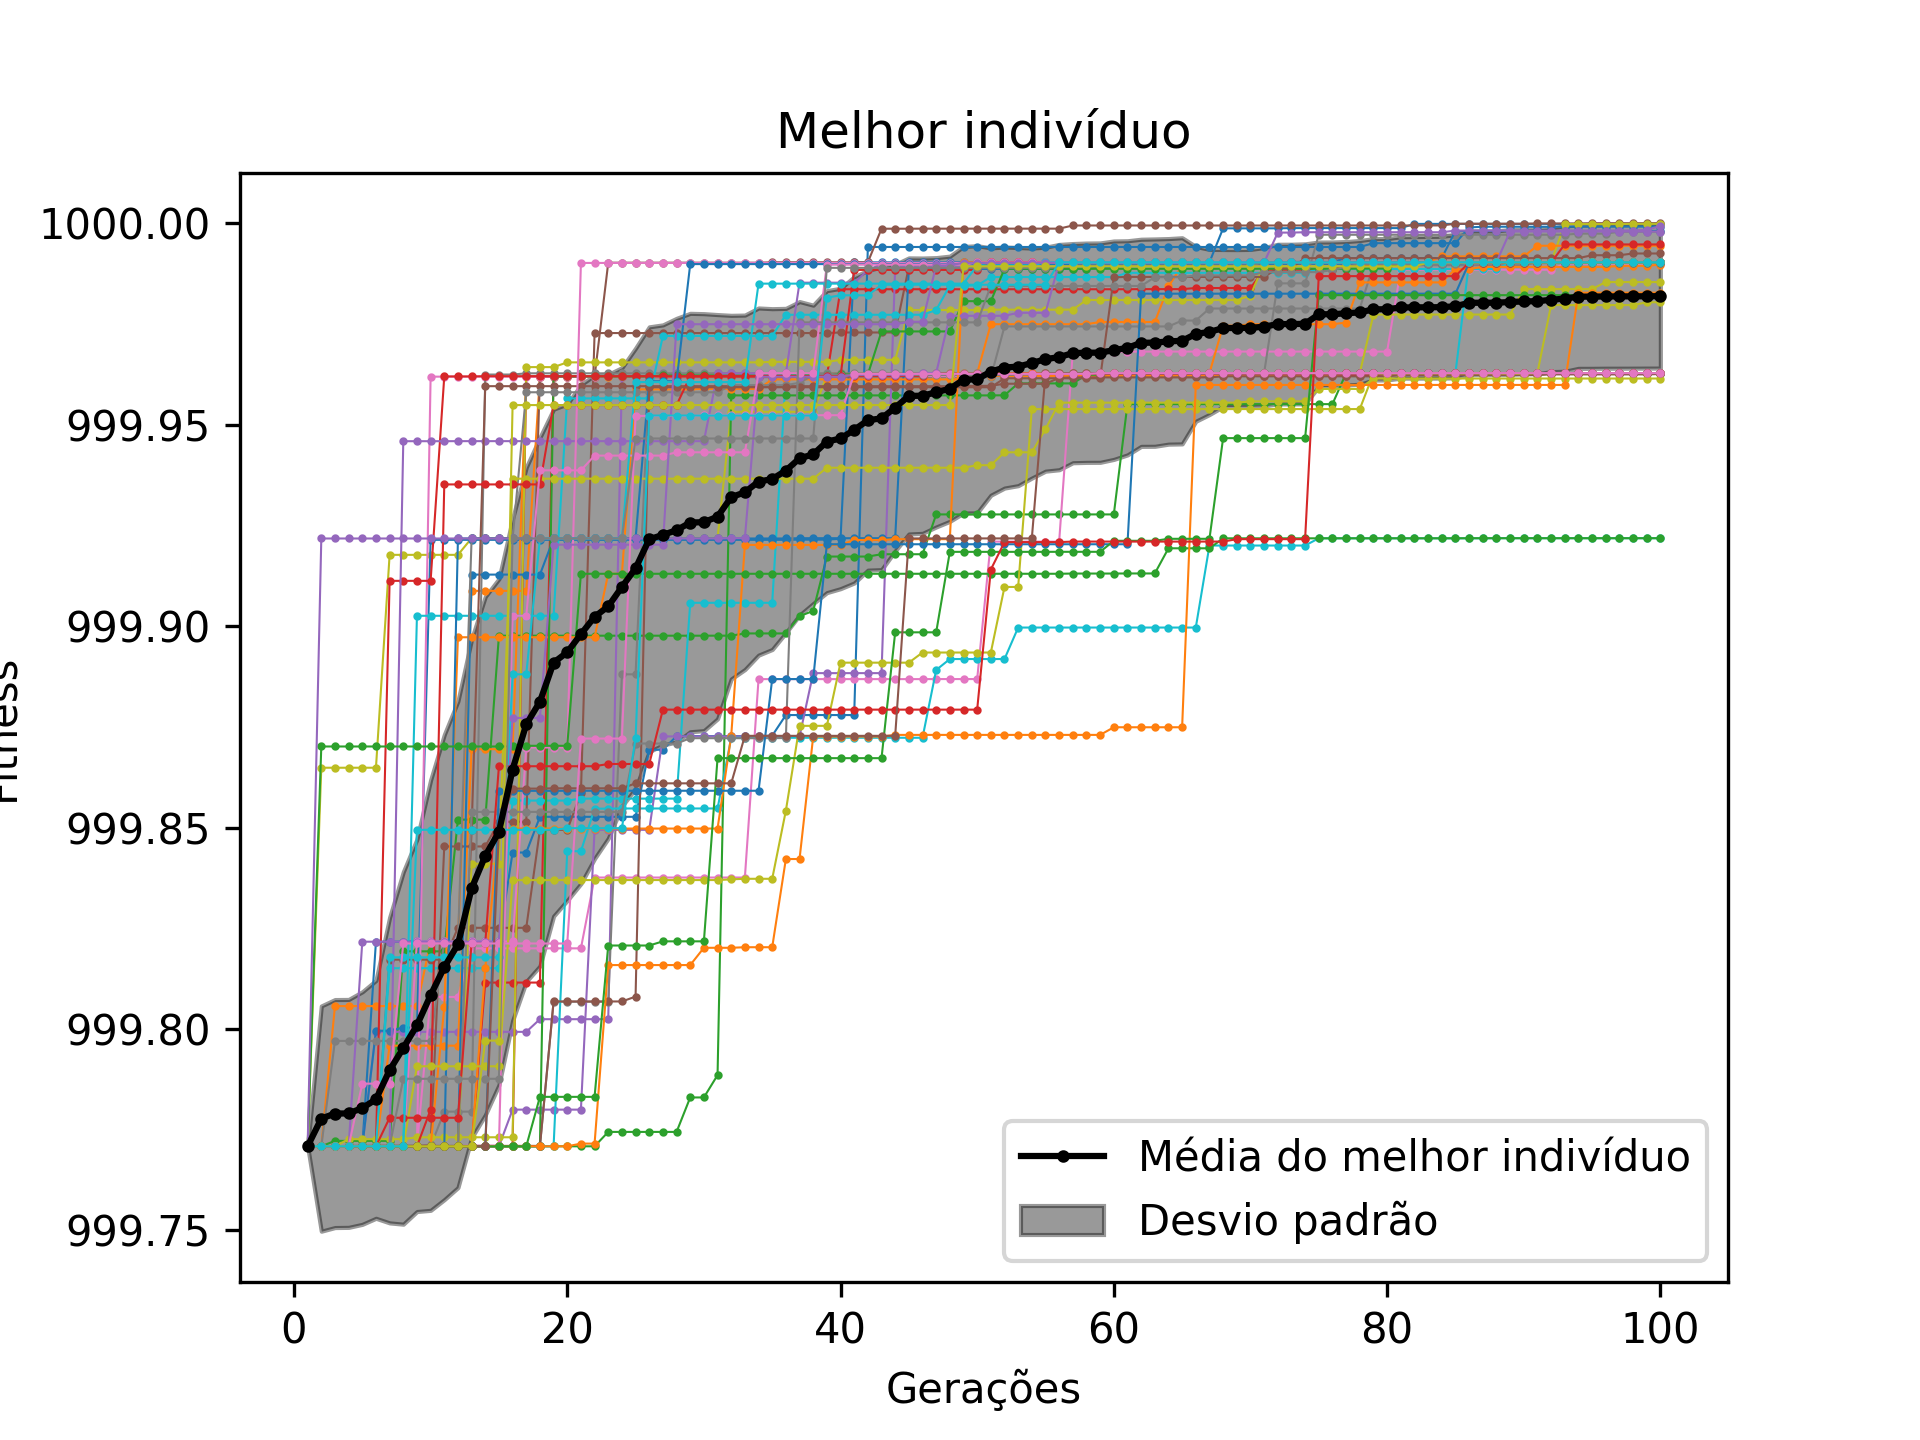
\includegraphics[width=1\textwidth]{sec-01/f6e_ss_fitness_vs_gen_best}
			\caption{Melhores indíviduos de todos os experimentos ao longo das gerações.
			Em preto é mostrado o comportamento médio dos 50 experimentos. }
		\end{subfigure}
		\hfill
		\begin{subfigure}{.45\textwidth}
			\centering
			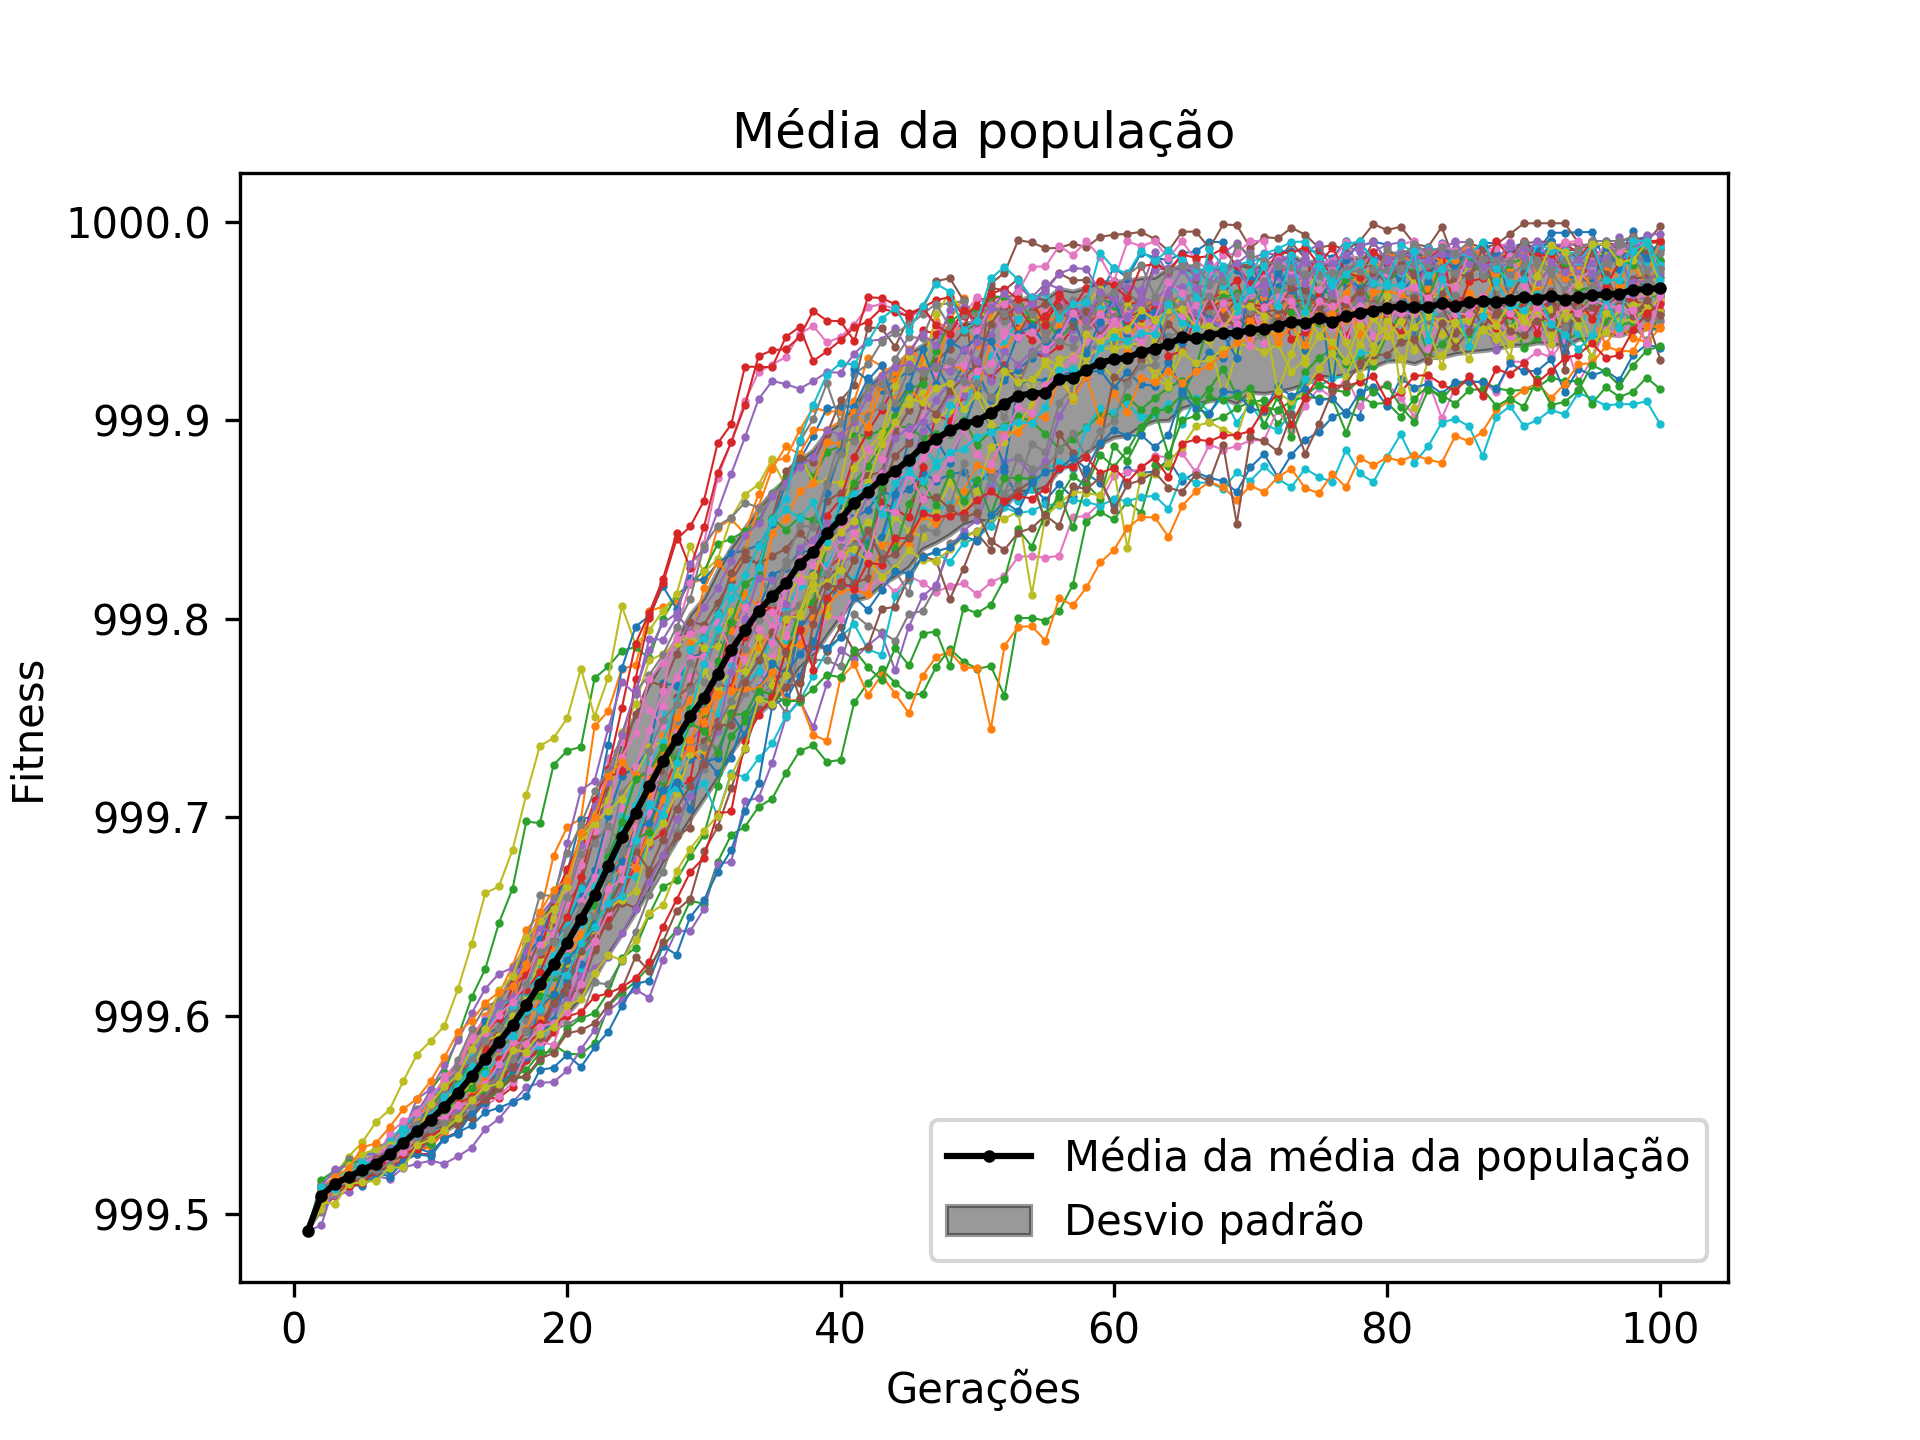
\includegraphics[width=1\textwidth]{sec-01/f6e_ss_fitness_vs_gen_pop}
			\caption{Média da população de todos os experimentos ao longo das gerações.
			Em preto é mostrado o comportamento médio dos 50 experimentos.}
		\end{subfigure}
		\caption{Resultados obtidos para a função $f6_{elevada}$ com estado estacionário de 20\% referentes ao teste 4 da tabela~\ref{tab:f6_stationary}}
	\end{figure}